%%%%%%%%%%%%%%%%%%%%%%%%%%%%%%%%%%%%%%%%%
% Wenneker Assignment
% LaTeX Template
% Version 2.0 (12/1/2019)
%
% This template originates from:
% http://www.LaTeXTemplates.com
%
% Authors:
% Vel (vel@LaTeXTemplates.com)
% Frits Wenneker
%
% License:
% CC BY-NC-SA 3.0 (http://creativecommons.org/licenses/by-nc-sa/3.0/)
% 
%%%%%%%%%%%%%%%%%%%%%%%%%%%%%%%%%%%%%%%%%

%----------------------------------------------------------------------------------------
%	PACKAGES AND OTHER DOCUMENT CONFIGURATIONS
%----------------------------------------------------------------------------------------

\documentclass[11pt]{scrartcl} % Font size

%%%%%%%%%%%%%%%%%%%%%%%%%%%%%%%%%%%%%%%%%
% Wenneker Assignment
% Structure Specification File
% Version 2.0 (12/1/2019)
%
% This template originates from:
% http://www.LaTeXTemplates.com
%
% Authors:
% Vel (vel@LaTeXTemplates.com)
% Frits Wenneker
%
% License:
% CC BY-NC-SA 3.0 (http://creativecommons.org/licenses/by-nc-sa/3.0/)
% 
%%%%%%%%%%%%%%%%%%%%%%%%%%%%%%%%%%%%%%%%%

%----------------------------------------------------------------------------------------
%	PACKAGES AND OTHER DOCUMENT CONFIGURATIONS
%----------------------------------------------------------------------------------------

\usepackage{amsmath, amsfonts, amsthm} % Math packages

\usepackage{listings} % Code listings, with syntax highlighting

\usepackage[english]{babel} % English language hyphenation

\usepackage{graphicx} % Required for inserting images
\graphicspath{{Figures/}{./}} % Specifies where to look for included images (trailing slash required)

\usepackage{booktabs} % Required for better horizontal rules in tables

\numberwithin{equation}{section} % Number equations within sections (i.e. 1.1, 1.2, 2.1, 2.2 instead of 1, 2, 3, 4)
\numberwithin{figure}{section} % Number figures within sections (i.e. 1.1, 1.2, 2.1, 2.2 instead of 1, 2, 3, 4)
\numberwithin{table}{section} % Number tables within sections (i.e. 1.1, 1.2, 2.1, 2.2 instead of 1, 2, 3, 4)

\setlength\parindent{0pt} % Removes all indentation from paragraphs

\usepackage{enumitem} % Required for list customisation
\setlist{noitemsep} % No spacing between list items

%----------------------------------------------------------------------------------------
%	DOCUMENT MARGINS
%----------------------------------------------------------------------------------------

\usepackage{geometry} % Required for adjusting page dimensions and margins

\geometry{
	paper=a4paper, % Paper size, change to letterpaper for US letter size
	top=2.5cm, % Top margin
	bottom=3cm, % Bottom margin
	left=3cm, % Left margin
	right=3cm, % Right margin
	headheight=0.75cm, % Header height
	footskip=1.5cm, % Space from the bottom margin to the baseline of the footer
	headsep=0.75cm, % Space from the top margin to the baseline of the header
	%showframe, % Uncomment to show how the type block is set on the page
}

%----------------------------------------------------------------------------------------
%	FONTS
%----------------------------------------------------------------------------------------

\usepackage[utf8]{inputenc} % Required for inputting international characters
\usepackage[T1]{fontenc} % Use 8-bit encoding

\usepackage{fourier} % Use the Adobe Utopia font for the document

%----------------------------------------------------------------------------------------
%	SECTION TITLES
%----------------------------------------------------------------------------------------

\usepackage{sectsty} % Allows customising section commands

\sectionfont{\vspace{6pt}\centering\normalfont\scshape} % \section{} styling
\subsectionfont{\normalfont\bfseries} % \subsection{} styling
\subsubsectionfont{\normalfont\itshape} % \subsubsection{} styling
\paragraphfont{\normalfont\scshape} % \paragraph{} styling

%----------------------------------------------------------------------------------------
%	HEADERS AND FOOTERS
%----------------------------------------------------------------------------------------

\usepackage{scrlayer-scrpage} % Required for customising headers and footers

\ohead*{} % Right header
\ihead*{} % Left header
\chead*{} % Centre header

\ofoot*{} % Right footer
\ifoot*{} % Left footer
\cfoot*{\pagemark} % Centre footer
 % Include the file specifying the document structure and custom commands

%----------------------------------------------------------------------------------------
%	TITLE SECTION
%----------------------------------------------------------------------------------------

\title{	
	\normalfont\normalsize
	\textsc{University of Texas at Austin}\\ % Your university, school and/or department name(s)
	\vspace{25pt} % Whitespace
	\rule{\linewidth}{0.5pt}\\ % Thin top horizontal rule
	\vspace{20pt} % Whitespace
	{\huge NEU 380E Color Prediction}\\ % The assignment title
	\vspace{12pt} % Whitespace
	\rule{\linewidth}{2pt}\\ % Thick bottom horizontal rule
	\vspace{12pt} % Whitespace
}

\author{\LARGE Haoqi Wang (haoqiwang@utexas.edu, ID: hw9335)} % Your name

\date{\normalsize\today} % Today's date (\today) or a custom date

\bibliographystyle{unsrt}

%To insert subfigure
\usepackage{graphicx}
\usepackage{float} 
\usepackage{subfigure}

%To input math
%\usepackage{amsfonts}
\usepackage[colorlinks,linkcolor=blue]{hyperref}

\usepackage{listings}
\usepackage{color}

\definecolor{dkgreen}{rgb}{0,0.6,0}
\definecolor{gray}{rgb}{0.5,0.5,0.5}
\definecolor{mauve}{rgb}{0.58,0,0.82}

\usepackage{algorithm}
\usepackage{algorithmic}

\begin{document}

\maketitle % Print the title

%----------------------------------------------------------------------------------------
%	FIGURE EXAMPLE
%----------------------------------------------------------------------------------------

\section{Introduction}

This homework aims at applying neural network to recognize hand-written digits. This report illustrated the basic theory of neural network, including forward propagation, backward propagation, gradient descent, etc. Then, we built a neural network from scratch using sigmoid as activation function and softmax for multiclass classification. After that, we evaluated loss of training and testing data. We also changed the number of units of hidden layer to measure its influence on accuracy. Moreover, we utilized RuLU as another activation function to train neural network. Based on several expriments, we found that around 100 neurons in hidden layer can perform pretty well with accuracy more than 95\%. Comparing activation function of sigmoid and ReLU, we noticed that sigmoid behaves better.



%------------------------------------------------

%\bibliography{test}

%----------------------------------------------------------------------------------------
%	TEXT EXAMPLE
%----------------------------------------------------------------------------------------

\section{Methods}

\subsection{Prepare image}
convert 16 bits ppm image to 8 bits jpg image

Each value is divided by $2^8$ to transform to 8 bits image

construct csv files to store data

train image
use jit numba
15s an image
3s on pretest image
calculate contrast

\begin{equation}
C_X=\sqrt{\frac19\sum_{i=1}^9{(\frac{X_i-\overline X}{\overline X})}^2}
\label{contrast}
\end{equation}

%\begin{equation}
%C_R=\sqrt{\frac19\sum_{i=1}^9{(\frac{R_i-\overline R}{\overline R})}^2}
%\label{contrast_red}
%\end{equation}

%\begin{equation}
%C_G=\sqrt{\frac19\sum_{i=1}^9{(\frac{G_i-\overline G}{\overline G})}^2}
%\label{contrast_green}
%\end{equation}

%\begin{equation}
%C_B=\sqrt{\frac19\sum_{i=1}^9{(\frac{B_i-\overline B}{\overline B})}^2}
%\label{contrast_blue}
%\end{equation}

, where
\begin{equation}
\overline X=\frac19\sum_{i=1}^9X_i
\label{mean}
\end{equation}

and $X=R,\;G,\;B$

\begin{equation}
C_{G,B}=\frac12(C_G+C_B)
\label{contrast_GB}
\end{equation}

\begin{equation}
C_{R,B}=\frac12(C_R+C_B)
\label{contrast_RB}
\end{equation}

\begin{equation}
C_{R,G}=\frac12(C_R+C_G)
\label{contrast_RG}
\end{equation}

$256*256*10$
record in txt file

remove color
set the color channel matrix as 0

recover image
\begin{equation}
{\widehat R}_{opt}=GB(G,B,C_{G,B})
\end{equation}

\begin{equation}
{\widehat G}_{opt}=RB(R,B,C_{R,B})
\end{equation}

\begin{equation}
{\widehat B}_{opt}=RG(R,G,C_{R,G})
\end{equation}

compare image
calculate mse
\begin{equation}
MSE=\frac1{n_1n_2n_3}\sum_i^{n_1}\sum_j^{n_2}\sum_k^{n_3}{({\widehat x}_{ijk}-x_{ijk})}^2
\end{equation}
, where $n_1$ is the number of channels, $n_2$ and $n_3$are number of rows and columns of an image.

gamma correction
First the image is scaled to $I_{in}\in(0,1)$, then apply gamma correction
\begin{equation}
I_{out}=I_{in}^\gamma
\end{equation}
, where we choose $\gamma=1/2$. After the correction, it is then scaled back to display.


\subsection{Neural network}

\subsubsection{Forward propagation}

There are basically two equations for forward propagation.

\begin{equation}
z^{\lbrack l\rbrack}=W^{\lbrack l\rbrack}a^{\lbrack l-1\rbrack}+b^{\lbrack l\rbrack}
\label{fp1}
\end{equation}

,where $z^{\lbrack l\rbrack}\in\mathbb{R}^{n^{\lbrack l\rbrack}\times1}$, $W^{\lbrack l\rbrack}\in\mathbb{R}^{n^{\lbrack l\rbrack}\times n^{\lbrack l-1\rbrack}}$, $b^{\lbrack l\rbrack}\in\mathbb{R}^{n^{\lbrack l\rbrack}\times1}$, $[l]$ is the index of layer and we have $L$ layers in total, $n^{\lbrack l\rbrack}$ is the number of units in $l$th layer. And

\begin{equation}
a^{\lbrack l\rbrack}=g^{\lbrack l\rbrack}(z^{\lbrack l\rbrack})
\label{fp2}
\end{equation}

, where $g^{\lbrack l\rbrack}$ is the activation function of $l$th layer. There are many choices activation functions, including sigmoid funciton

\begin{equation}
g(z)=\frac1{1+e^{-z}}
\end{equation}

Rectified Linear Unit (ReLU)

\begin{equation}
g(z)=max(0,z)
\end{equation}

For the last layer, we have the equations

\begin{equation}
z^{\lbrack L\rbrack}=W^{\lbrack L\rbrack}a^{\lbrack L-1\rbrack}+b^{\lbrack L\rbrack}
\end{equation}

\begin{equation}
\widehat y=a^{\lbrack L\rbrack}=g^{\lbrack L\rbrack}(z^{\lbrack L\rbrack})
\end{equation}

%\begin{equation}
%\mathcal L=f(a^{\lbrack L\rbrack})
%\end{equation}

\begin{equation}
\mathcal L=f(\widehat y)
\end{equation}

, where $f$ is loss function. Suppose we have $m$ samples in total, the loss function for $i$th sample can be written as 

\begin{equation}
\mathcal L^{(i)}=f(a^{\lbrack L\rbrack(i)})
\end{equation}

and the cost function $C$ is the average of the loss functions of the entire training set.

\begin{equation}
C=\frac1m\sum_{i=1}^m\mathcal L^{(i)}
\label{fp3}
\end{equation}

There are mnay kinds of loss functions, like quadratic loss function

\begin{equation}
\mathcal L=\frac12\sum_{k=1}^{n^{\lbrack L\rbrack}}(\widehat y_k-y_k)^{2}
\end{equation}

and cross entropy loss

\begin{equation}
\mathcal L=-\sum_{k=1}^{n^{\lbrack L\rbrack}}y_k\log{\widehat y}_k
\end{equation}

where $y_k$ is ground truth.


\subsubsection{Backward propagation}

After computing cost function, we will use backward propagation to update parameters. For each term, equations \eqref{fp1} and \eqref{fp2} can be written as

\begin{equation}
z_i^{\lbrack l\rbrack}=\sum_j^{n^{\lbrack l-1\rbrack}}W_{ij}^{\lbrack l\rbrack}a_j^{\lbrack l-1\rbrack}+b_i^{\lbrack l\rbrack}
\end{equation}

\begin{equation}
a_i^{\lbrack l\rbrack}=g^{\lbrack l\rbrack}(z_i^{\lbrack l\rbrack})
\end{equation}

Apparently, we can have the folowing partial derivatives

\begin{equation}
\left\{\begin{array}
{l}\frac{\partial z_i^{\lbrack l\rbrack}}{\partial W_{ij}^{\lbrack l\rbrack}}=a_j^{\lbrack l-1\rbrack}
\\\frac{\partial z_i^{\lbrack l\rbrack}}{\partial a_j^{\lbrack l-1\rbrack}}=W_{ij}^{\lbrack l\rbrack}
\\\frac{\partial z_i^{\lbrack l\rbrack}}{\partial b_i^{\lbrack l\rbrack}}=1
\\\frac{\partial a_i^{\lbrack l\rbrack}}{\partial z_i^{\lbrack l\rbrack}}=g^{{\lbrack l\rbrack}'}(z_i^{\lbrack l\rbrack})
\end{array}\right.
\end{equation}

, which will be utilized in the following derivations.

Here we define

\begin{equation}
\delta_i^{\lbrack l\rbrack}=\frac{\partial C}{\partial z_i^{\lbrack l\rbrack}}
\end{equation}

So 

\begin{equation}
\delta_i^{\lbrack L\rbrack}=\frac{\partial\ C}{\partial z_i^{\lbrack L\rbrack}}=\frac{\partial\ C}{\partial a_i^{\lbrack L\rbrack}}\frac{\partial a_i^{\lbrack L\rbrack}}{\partial z_i^{\lbrack L\rbrack}}=\frac{\partial\ C}{\partial a_i^{\lbrack L\rbrack}}g^{{\lbrack L\rbrack}'}(z_i^{\lbrack L\rbrack})
\end{equation}

, which can be vectorized as 

\begin{equation}
\delta^{\lbrack L\rbrack}=\nabla_{a^{\lbrack L\rbrack}}C\odot g^{{\lbrack L\rbrack}'}(z^{\lbrack L\rbrack})
\label{bp1}
\end{equation}

And 

\begin{equation}
\begin{split}
\delta_i^{\lbrack l\rbrack} &=\frac{\partial C}{\partial z_i^{\lbrack l\rbrack}} \\
&=\frac{\partial C}{\partial a_i^{\lbrack l\rbrack}}\frac{\partial a_i^{\lbrack l\rbrack}}{\partial z_i^{\lbrack l\rbrack}} \\
&=(\sum_{j=1}^{n^{\lbrack l+1\rbrack}}\frac{\partial C}{\partial z_j^{\lbrack l+1\rbrack}}\frac{\partial z_j^{\lbrack l+1\rbrack}}{\partial a_i^{\lbrack l\rbrack}})\frac{\partial a_i^{\lbrack l\rbrack}}{\partial z_i^{\lbrack l\rbrack}} \\
&=(\sum_{j=1}^{n^{\lbrack l+1\rbrack}}\delta_j^{\lbrack l+1\rbrack}W_{ji}^{\lbrack l+1\rbrack})g^{{\lbrack l\rbrack}'}(z_i^{\lbrack l\rbrack})
\end{split}
\end{equation}

, which can be vectorized as 

\begin{equation}
\delta^{\lbrack l\rbrack}=(W^{{\lbrack l+1\rbrack}^T}\delta^{\lbrack l+1\rbrack})\odot g^{{\lbrack l\rbrack}'}(z^{\lbrack l\rbrack})
\label{bp2}
\end{equation}

And

\begin{equation}
\begin{split}
\frac{\partial C}{\partial b_i^{\lbrack l\rbrack}} &=\frac{\partial C}{\partial z_i^{\lbrack l\rbrack}}\frac{\partial z_i^{\lbrack l\rbrack}}{\partial b_i^{\lbrack l\rbrack}} \\
&=\delta_i^{\lbrack l\rbrack}
\end{split}
\end{equation}

, which can be vectorized as 

\begin{equation}
\frac{\partial C}{\partial b^{\lbrack l\rbrack}}=\delta^{\lbrack l\rbrack}
\label{bp3}
\end{equation}

And

\begin{equation}
\begin{split}
\frac{\partial C}{\partial W_{ij}^{\lbrack l\rbrack}}&=\frac{\partial C}{\partial z_i^{\lbrack l\rbrack}}\frac{\partial z_i^{\lbrack l\rbrack}}{\partial W_{ij}^{\lbrack l\rbrack}} \\
&=\delta_i^{\lbrack l\rbrack}a_j^{\lbrack l-1\rbrack}
\end{split}
\end{equation}

, which can be vectorized as 

\begin{equation}
\frac{\partial C}{\partial W^{\lbrack l\rbrack}}=\delta^{\lbrack l\rbrack}a^{{\lbrack l-1\rbrack}^T}
\label{bp4}
\end{equation}

\eqref{bp1}, \eqref{bp2}, \eqref{bp3}, \eqref{bp4} are 4 basic equations in back propagation. For each iteration, the parameters are updated as 

\begin{equation}
W^{\lbrack l\rbrack}=W^{\lbrack l\rbrack}-\eta \frac{\partial C}{\partial W^{\lbrack l\rbrack}}
\label{bp5}
\end{equation}

\begin{equation}
b^{\lbrack l\rbrack}=b^{\lbrack l\rbrack}-\eta \frac{\partial C}{\partial b^{\lbrack l\rbrack}}
\label{bp6}
\end{equation}

, where $\eta$ is learning rate.

\subsubsection{Algorithm}
The algorithm of training a neural network is the following.
\begin{algorithm}
	\caption{Neural network}
	\label{alg:A}
	\begin{algorithmic}
		\STATE {1. \textbf{Initialization}: Initialize $W^{[l]}$, $b^{[l]}$ and activation functions for each layer} 
		\STATE {2. \textbf{Forward propagation}: For $l=1,2,...,L$, apply \eqref{fp1} and \eqref{fp2} toward \eqref{fp3}}
		\STATE {3. \textbf{Output error}: Compute cost of last layer according to \eqref{bp1}}
		\STATE {4. \textbf{Backpropagate error}: Compute cost for each layer according to \eqref{bp2}}
		\STATE {5. \textbf{Update parameters}: Update $W^{[l]}$, $b^{[l]}$ according to \eqref{bp3}, \eqref{bp4}, \eqref{bp5}, \eqref{bp6}}
	\end{algorithmic}
\end{algorithm}

\subsection{Gradient descent}

Basically there are 3 ways of gradient descent. The equation \eqref{fp3} is gradient descent, in which case we add all the loss of the entire training set. This method can give us the optimal move of descent, while it can be time consuming. If we only consider one sample, i.e. $m=1$, this is stochastic gradient descent (SGD). For batch gradient descent, we consider some samples a time for cost function. Generally we have two ways to judge whether the iteration stops or not, one is setting an iterations limit, another is we setting a threshold in advance and it stops when the cost meets the requirement.

\subsection{Softmax and cross entropy}

We applied softmax function for multiclass classification, which is 

\begin{equation}
\widehat{y_i}=a_i^{\lbrack L\rbrack}=\frac{e^{z_i^{\lbrack L\rbrack}}}{{\displaystyle\sum_j^{n^{\lbrack L\rbrack}}}e^{z_j^{\lbrack L\rbrack}}}
\end{equation}

So we have 

\begin{equation}
\frac{\partial a_i^{\lbrack L\rbrack}}{\partial z_j^{\lbrack L\rbrack}}=a_i^{\lbrack L\rbrack}(\delta_{ij}-a_j^{\lbrack L\rbrack})
\end{equation}

, where $\delta_{ij}$ is Kronecker delta. So

\begin{equation}
\begin{split}
\frac{\partial\mathcal L}{\partial z_j^{\lbrack L\rbrack}}&=-\frac\partial{\partial z_j^{\lbrack L\rbrack}}\sum_{i=1}^{n^{\lbrack L\rbrack}}y_i\log a_i^{\lbrack L\rbrack} \\
&=-\sum_{i=1}^{n^{\lbrack L\rbrack}}y_i\frac{\partial{\log a_i^{\lbrack L\rbrack}}}{\partial {a_i^{\lbrack L\rbrack}}}\frac{\partial {a_i^{\lbrack L\rbrack}}}{\partial {z_j^{\lbrack L\rbrack}}} \\
&=-\sum_{i=1}^{n^{\lbrack L\rbrack}}y_i(\delta_{ij}-a_j^{\lbrack L\rbrack}) \\
&=a_j^{\lbrack L\rbrack}-y_j
\end{split}
\end{equation}

So 

\begin{equation}
\frac{\partial\mathcal L}{\partial z^{\lbrack L\rbrack}}=a^{\lbrack L\rbrack}-y
\end{equation}

\begin{equation}
\delta^{\lbrack L\rbrack}=\frac{\partial C}{\partial z^{\lbrack L\rbrack}}=\sum_{i=1}^{m}(a^{\lbrack L\rbrack (i)}-y^{(i)})
\end{equation}

Combing softmax and cross entropy, the $\delta^{\lbrack L\rbrack}$ is quite a simple form.

\subsection{Prediction}
After the neural network is trained, we input test images. The netwok will output the probabilities for each digit and the digit with the highest probability would be the prediction. Then it would be compared with the labels to acquire accuracy of our model.
%------------------------------------------------

%----------------------------------------------------------------------------------------
%	EQUATION EXAMPLES
%----------------------------------------------------------------------------------------

\section{Results}

\subsection{pre-test}

\ref{natural_forest_predicted_red}
\ref{natural_forest_predicted_green}
\ref{natural_forest_predicted_blue}
\ref{predicted color no contrast pre}
natural forest recover\ref{natural_forest_recover}

\begin{figure}[h] % [h] forces the figure to be output where it is defined in the code (it suppresses floating)
	\centering
	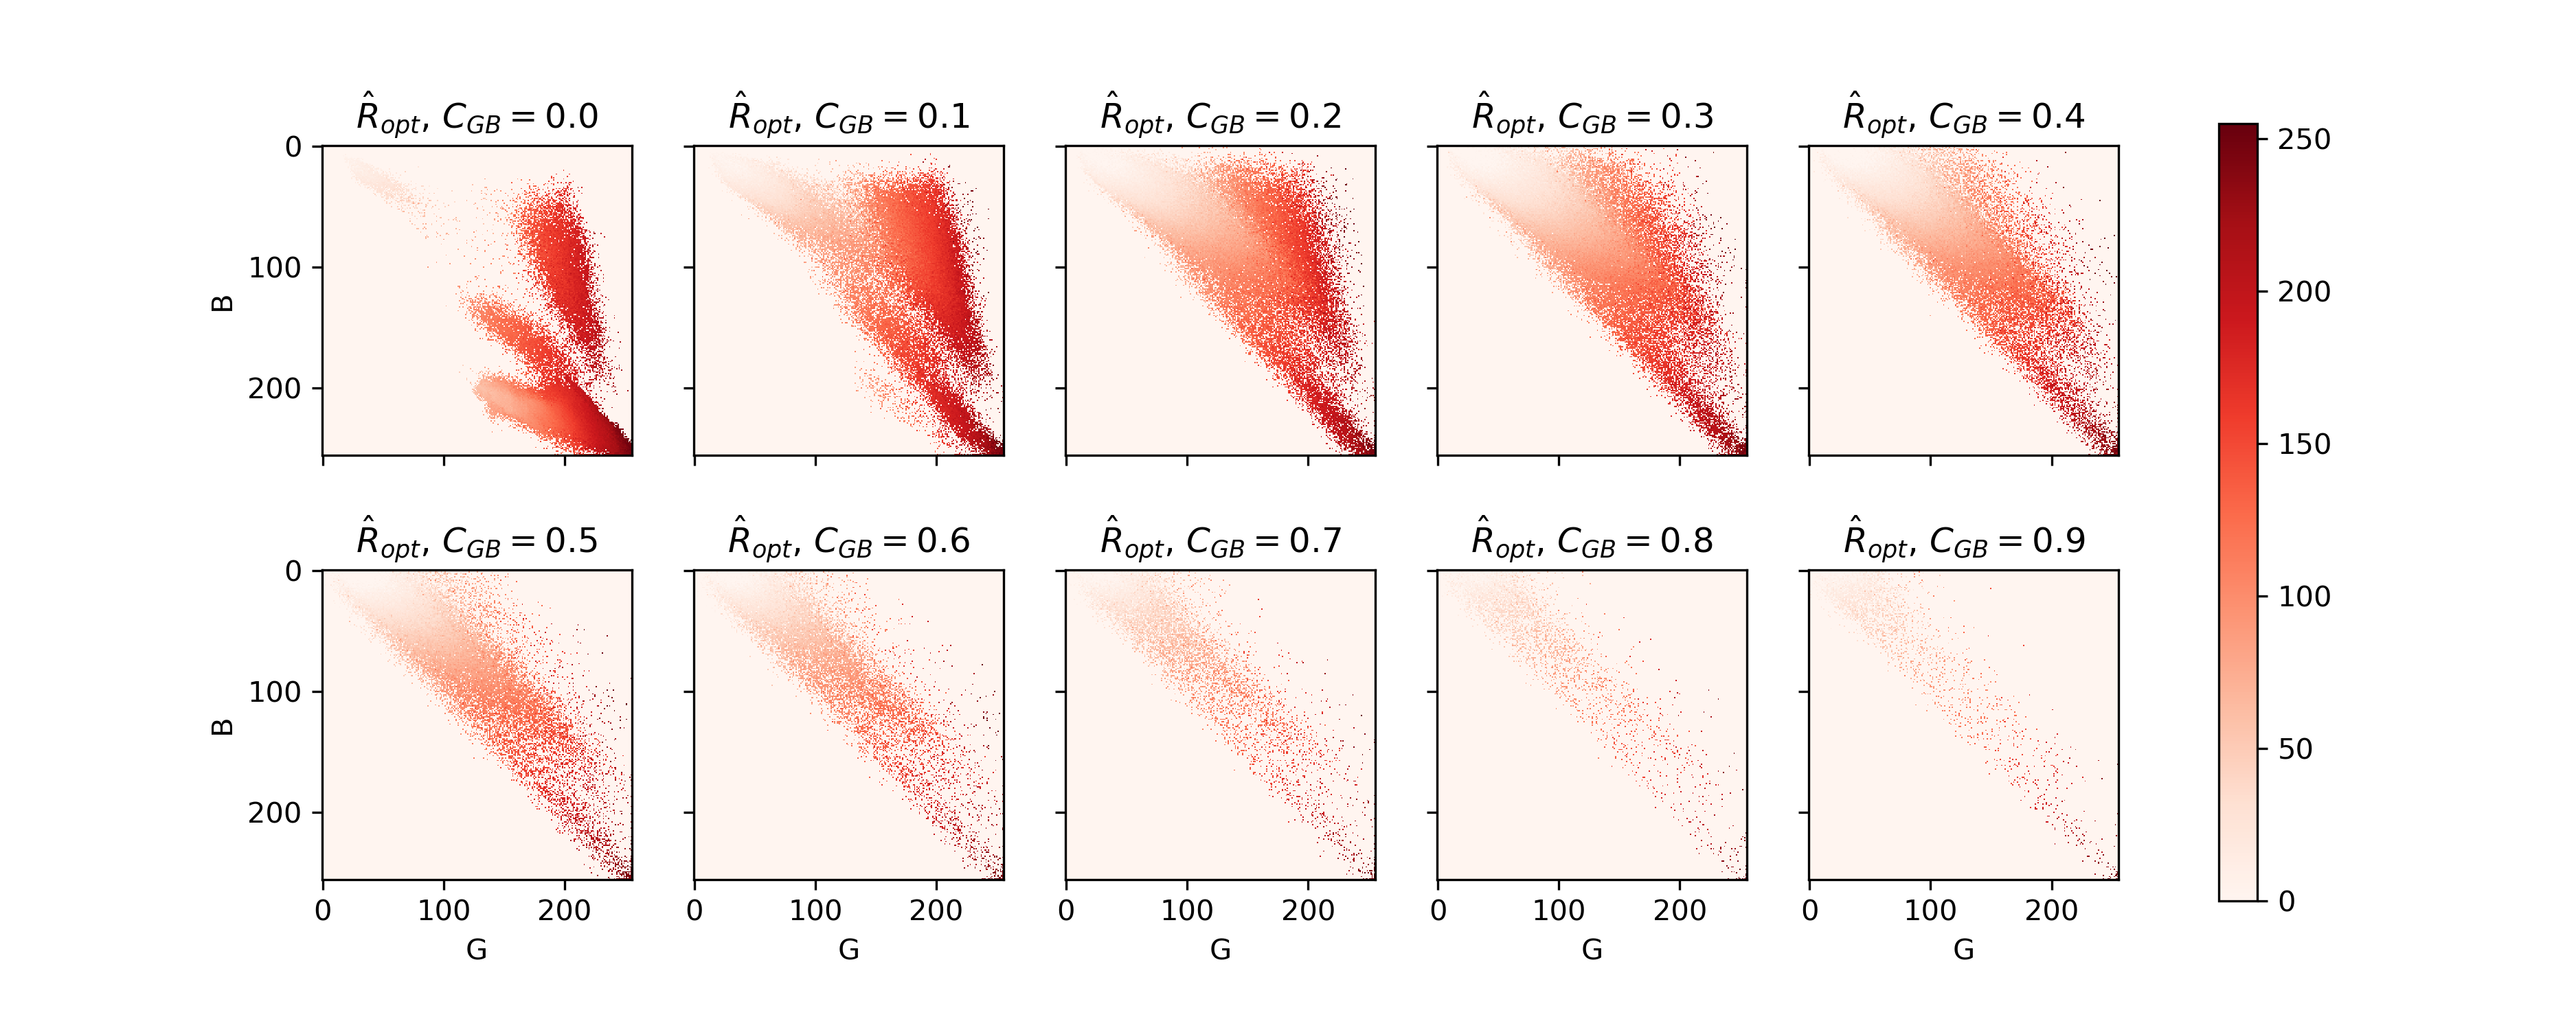
\includegraphics[width=1\columnwidth]{Figure/natural_forest_predicted_red} % Example image
	\caption{natural forest predicted red}
	\label{natural_forest_predicted_red}
\end{figure}

\begin{figure}[h] % [h] forces the figure to be output where it is defined in the code (it suppresses floating)
	\centering
	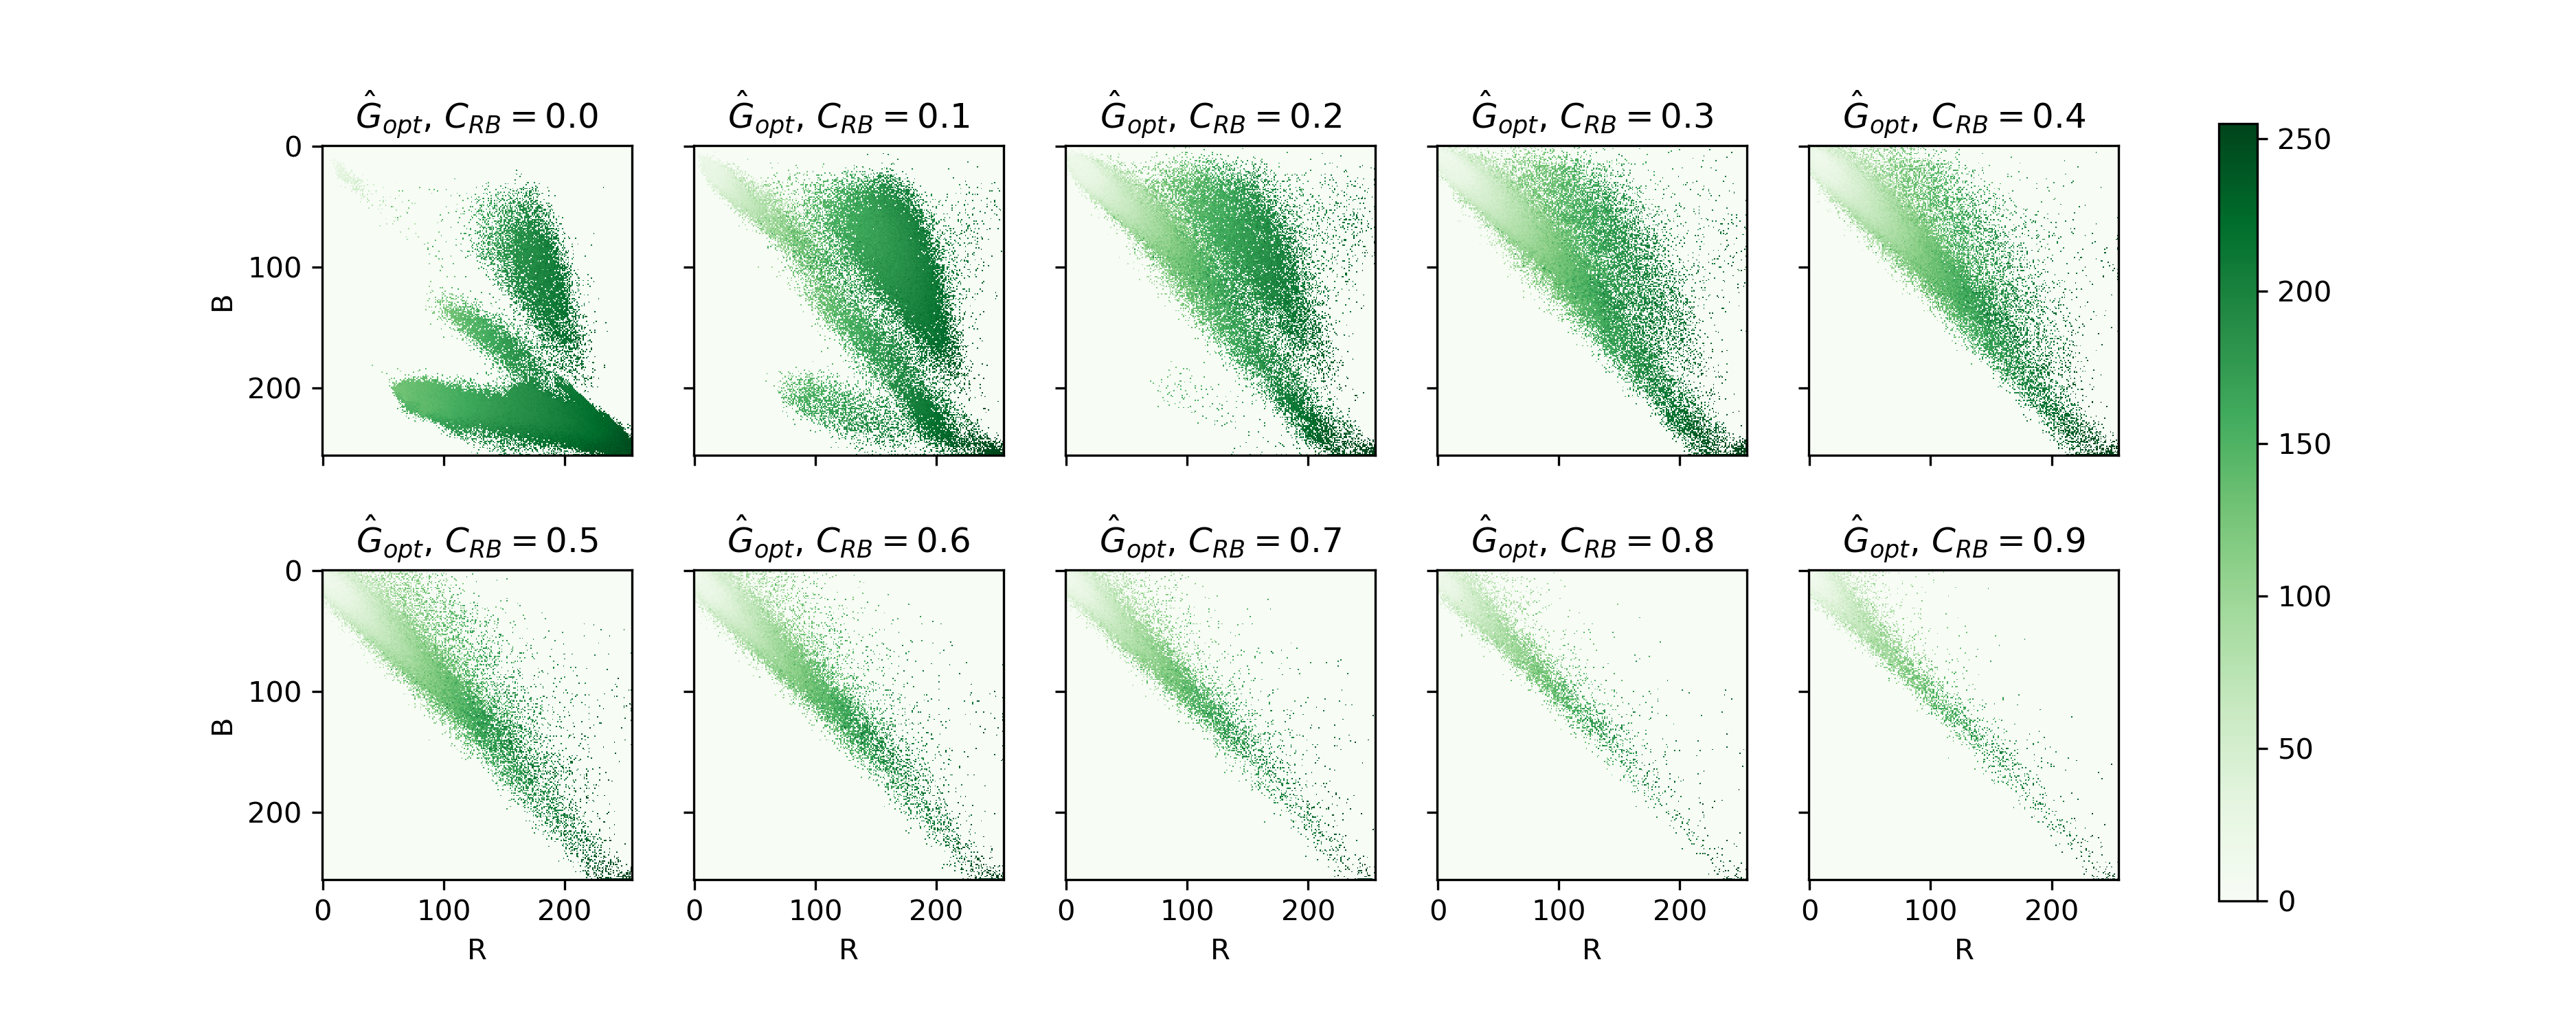
\includegraphics[width=1\columnwidth]{Figure/natural_forest_predicted_green} % Example image
	\caption{natural forest predicted green}
	\label{natural_forest_predicted_green}
\end{figure}

\begin{figure}[h] % [h] forces the figure to be output where it is defined in the code (it suppresses floating)
	\centering
	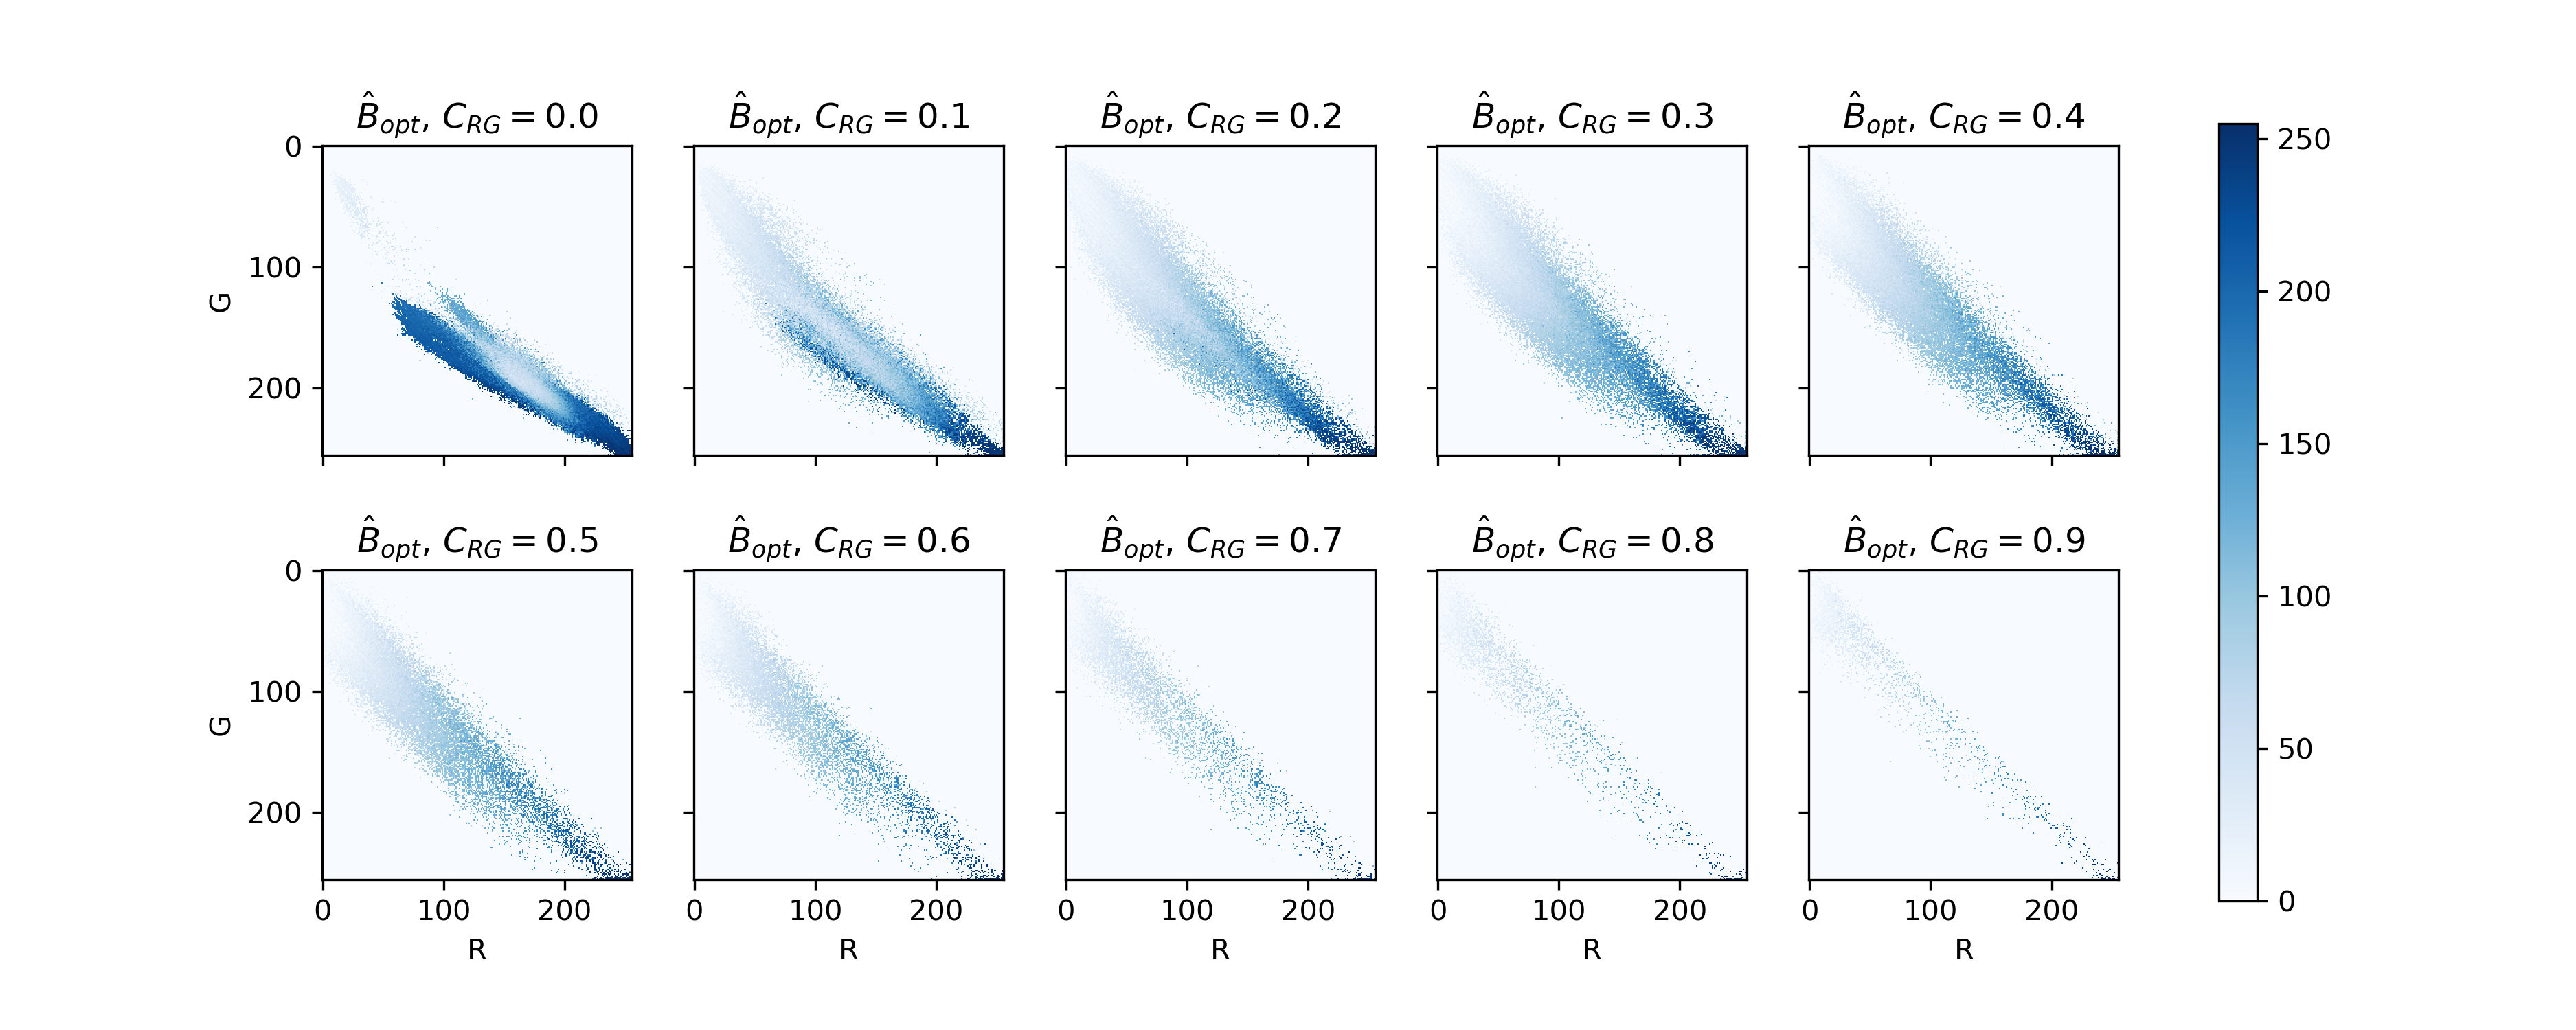
\includegraphics[width=1\columnwidth]{Figure/natural_forest_predicted_blue} % Example image
	\caption{natural forest predicted blue}
	\label{natural_forest_predicted_blue}
\end{figure}

\begin{figure}[H]
	\centering  %图片全局居中
	\subfigure[predicted red no contrast]{
		\label{predicted_red_no_contrast_pre}
		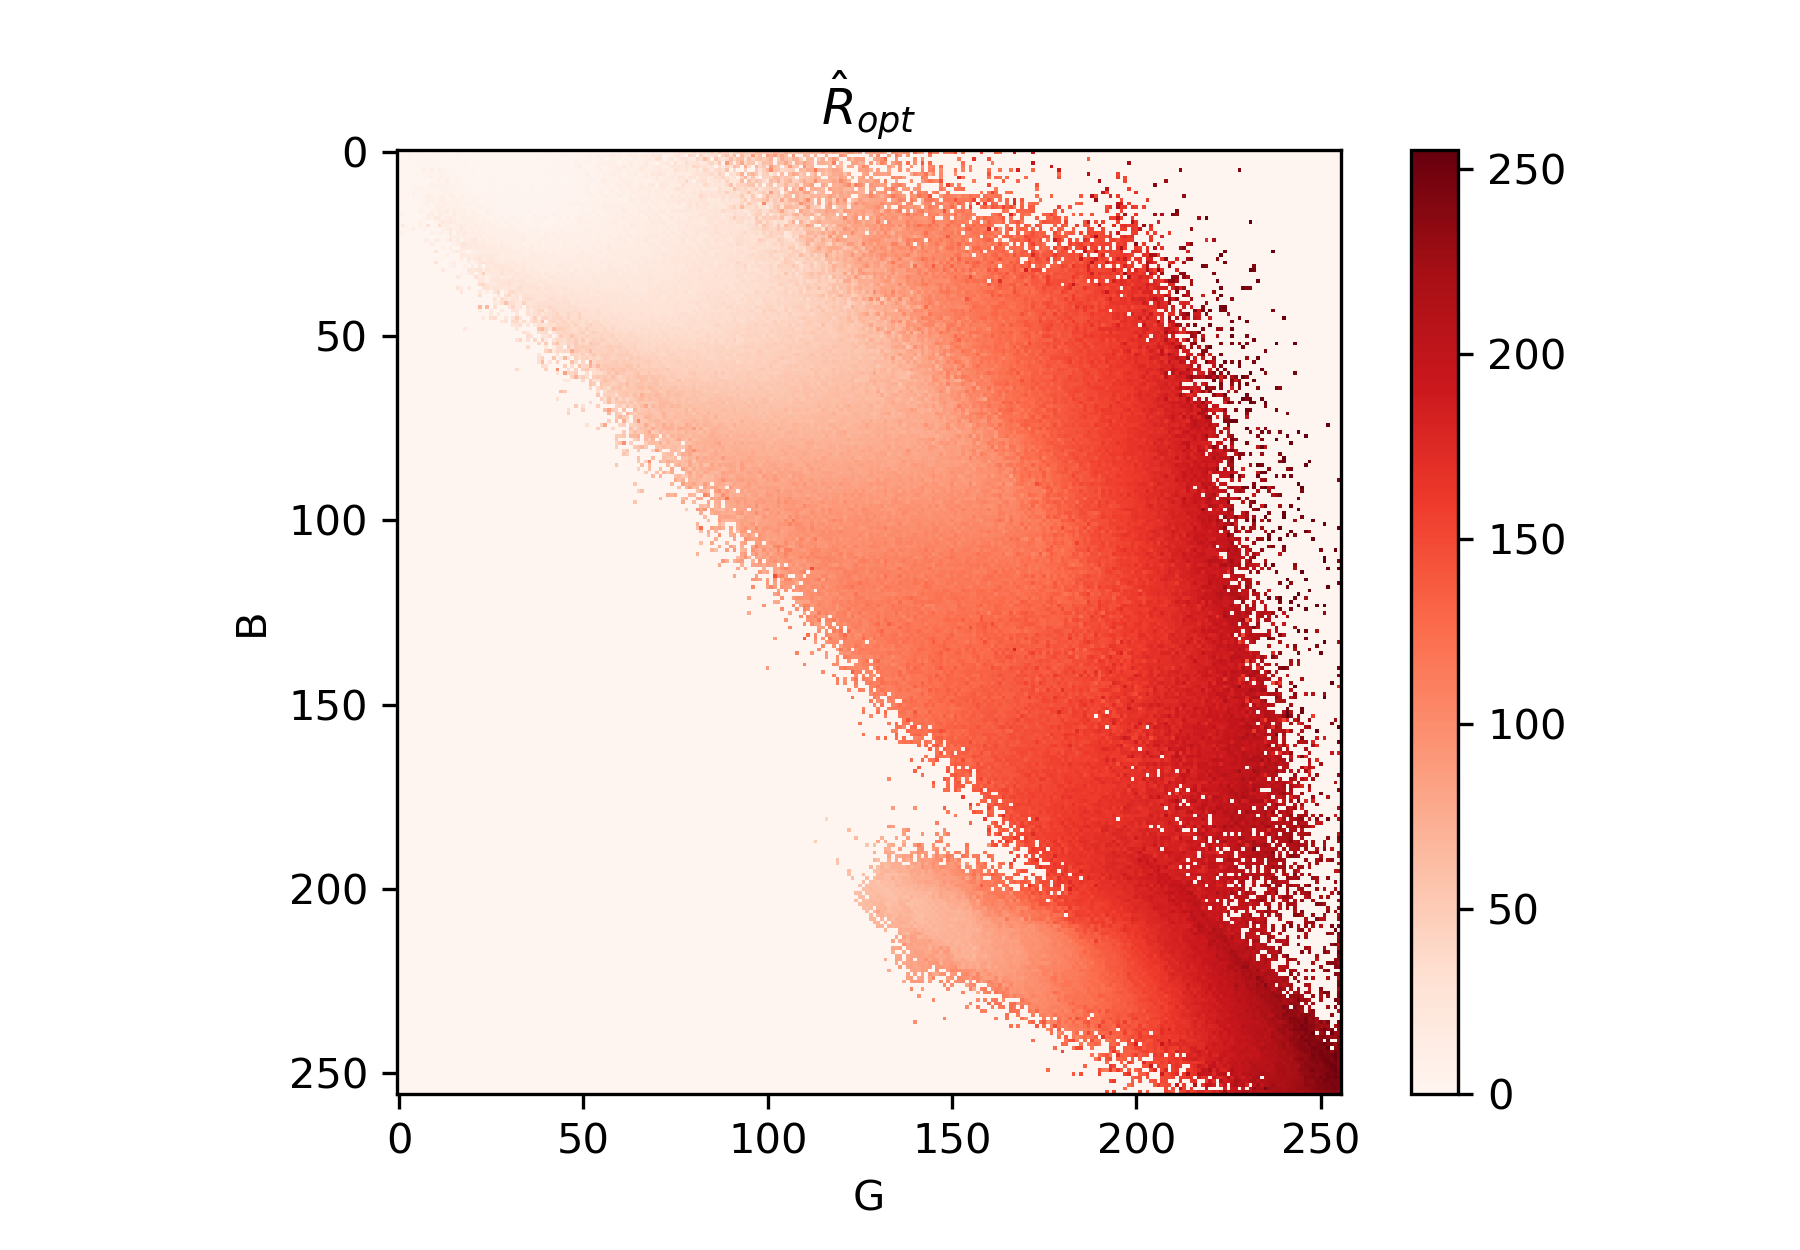
\includegraphics[width=0.32\textwidth]{Figure/predicted_red_no_contrast_pre}}
	\subfigure[predicted green no contrast pre]{
		\label{predicted_green_no_contrast_pre}
		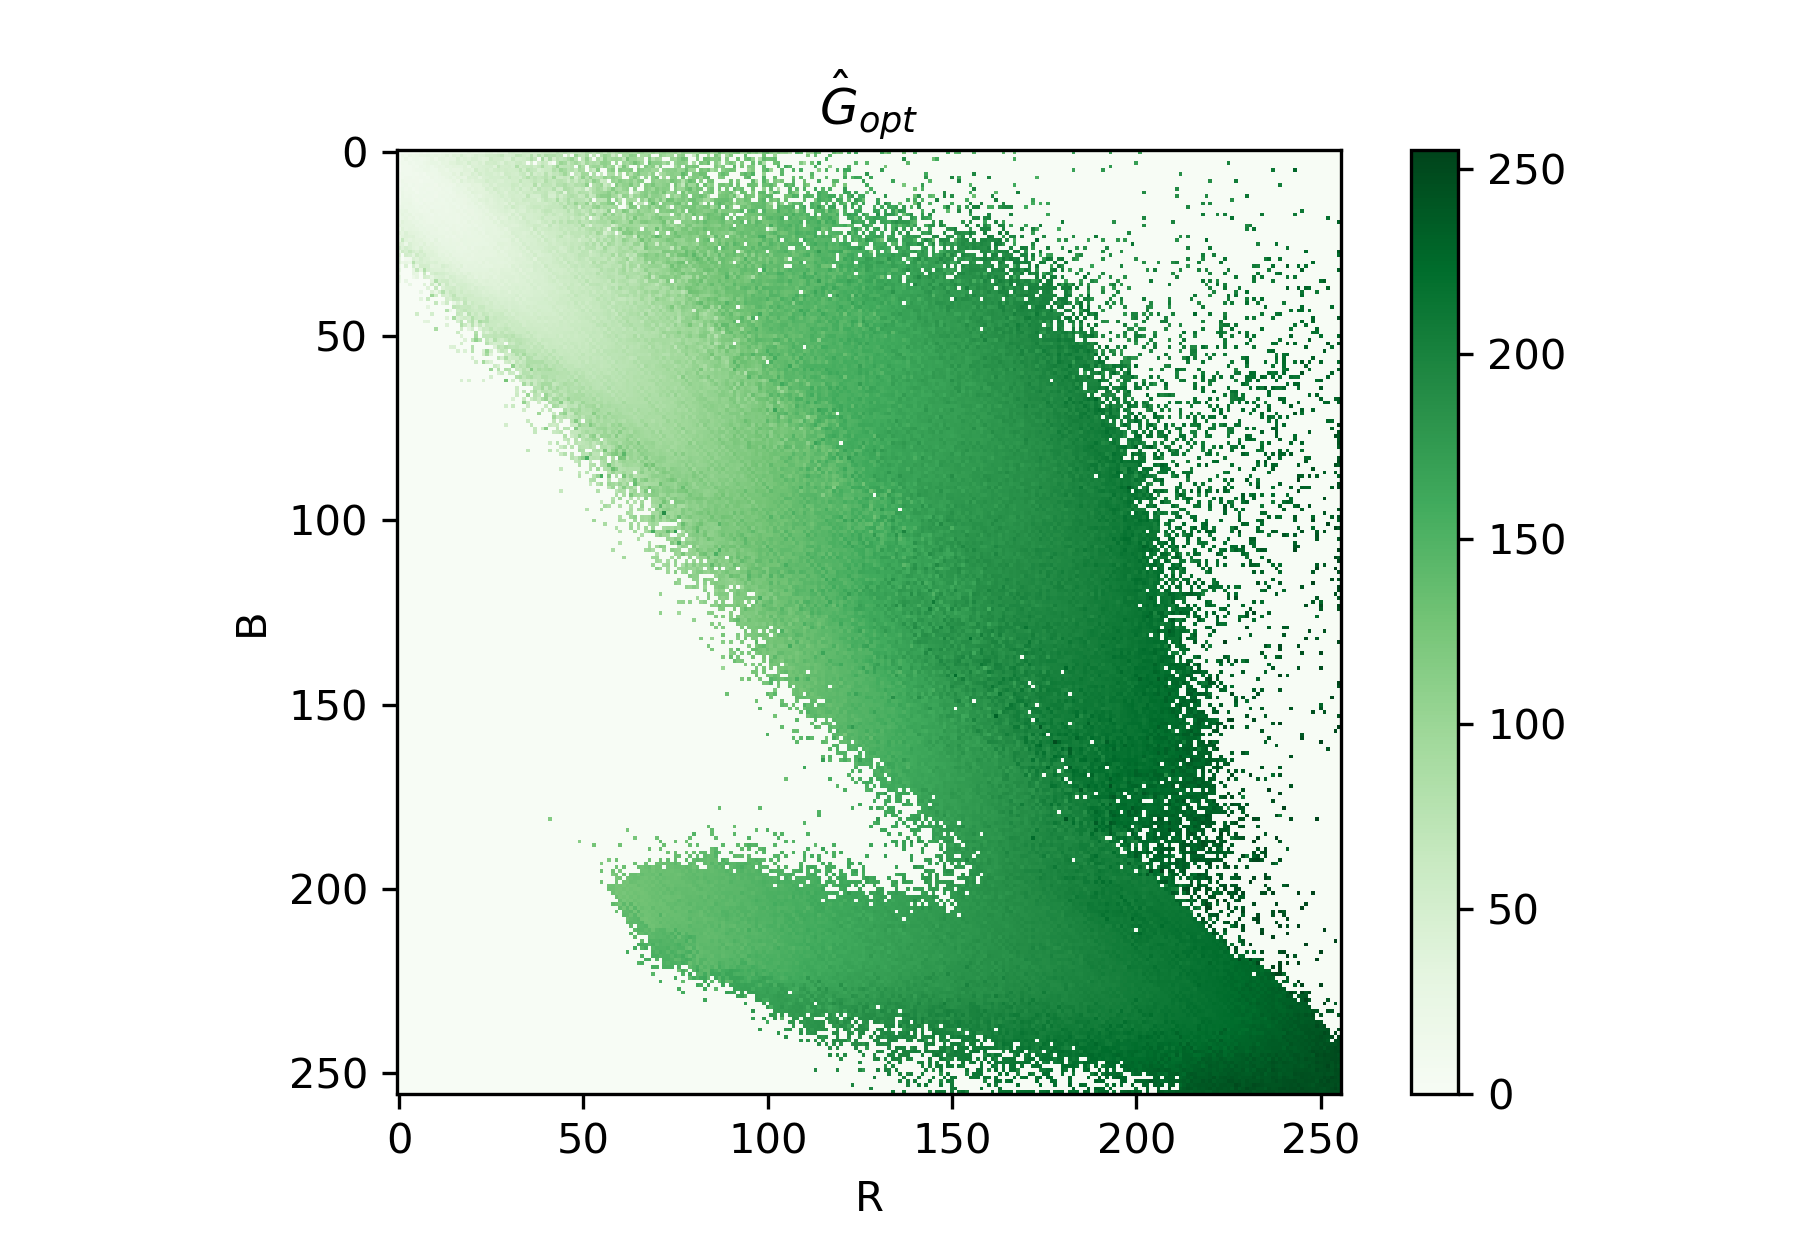
\includegraphics[width=0.32\textwidth]{Figure/predicted_green_no_contrast_pre}}
	\subfigure[predicted blue no contrast pre]{
		\label{predicted_blue_no_contrast_pre}
		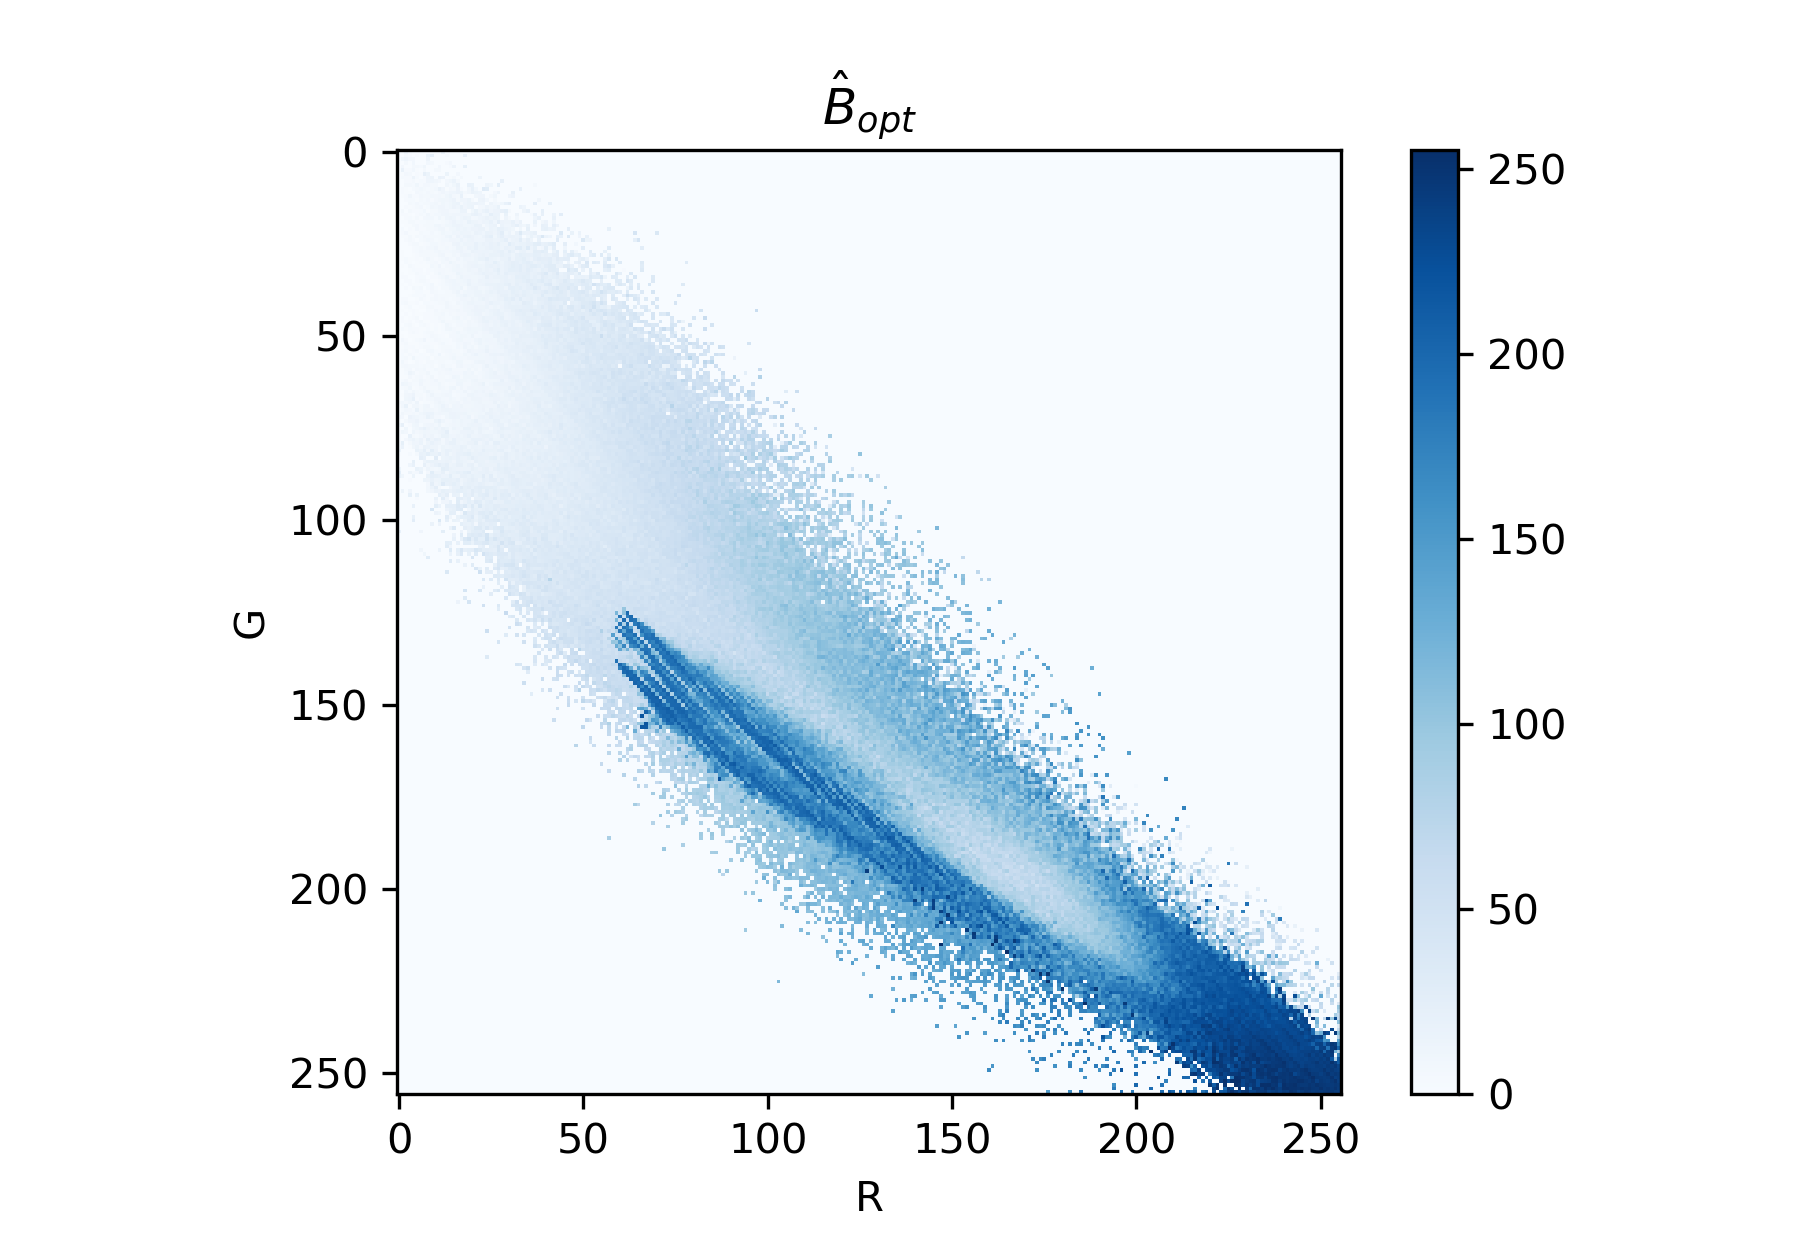
\includegraphics[width=0.32\textwidth]{Figure/predicted_blue_no_contrast_pre}}
	\caption{predicted color no contrast pre}
	\label{predicted color no contrast pre}
\end{figure}

%\begin{figure}[h] % [h] forces the figure to be output where it is defined in the code (it suppresses floating)
%	\centering
%	\includegraphics[width=1\columnwidth]{Figure/natural_forest_recover} % Example image
%	\caption{natural forest recover}
%	\label{natural_forest_recover}
%\end{figure}

\subsection{Record visualization}

Estimation of a missing color channel. Plots show the optimal estimate of the missing color value given the observed color values on the horizontal and vertical axes.

predicted red \ref{predicted red} 
predicted green\ref{predicted green}
predicted blue\ref{predicted blue}

predicted colors no contrast\ref{predicted color no contrast}
predicted colors no contrast surface plot\ref{predicted color no contrast surface plot}

\begin{figure}[h] % [h] forces the figure to be output where it is defined in the code (it suppresses floating)
	\centering
	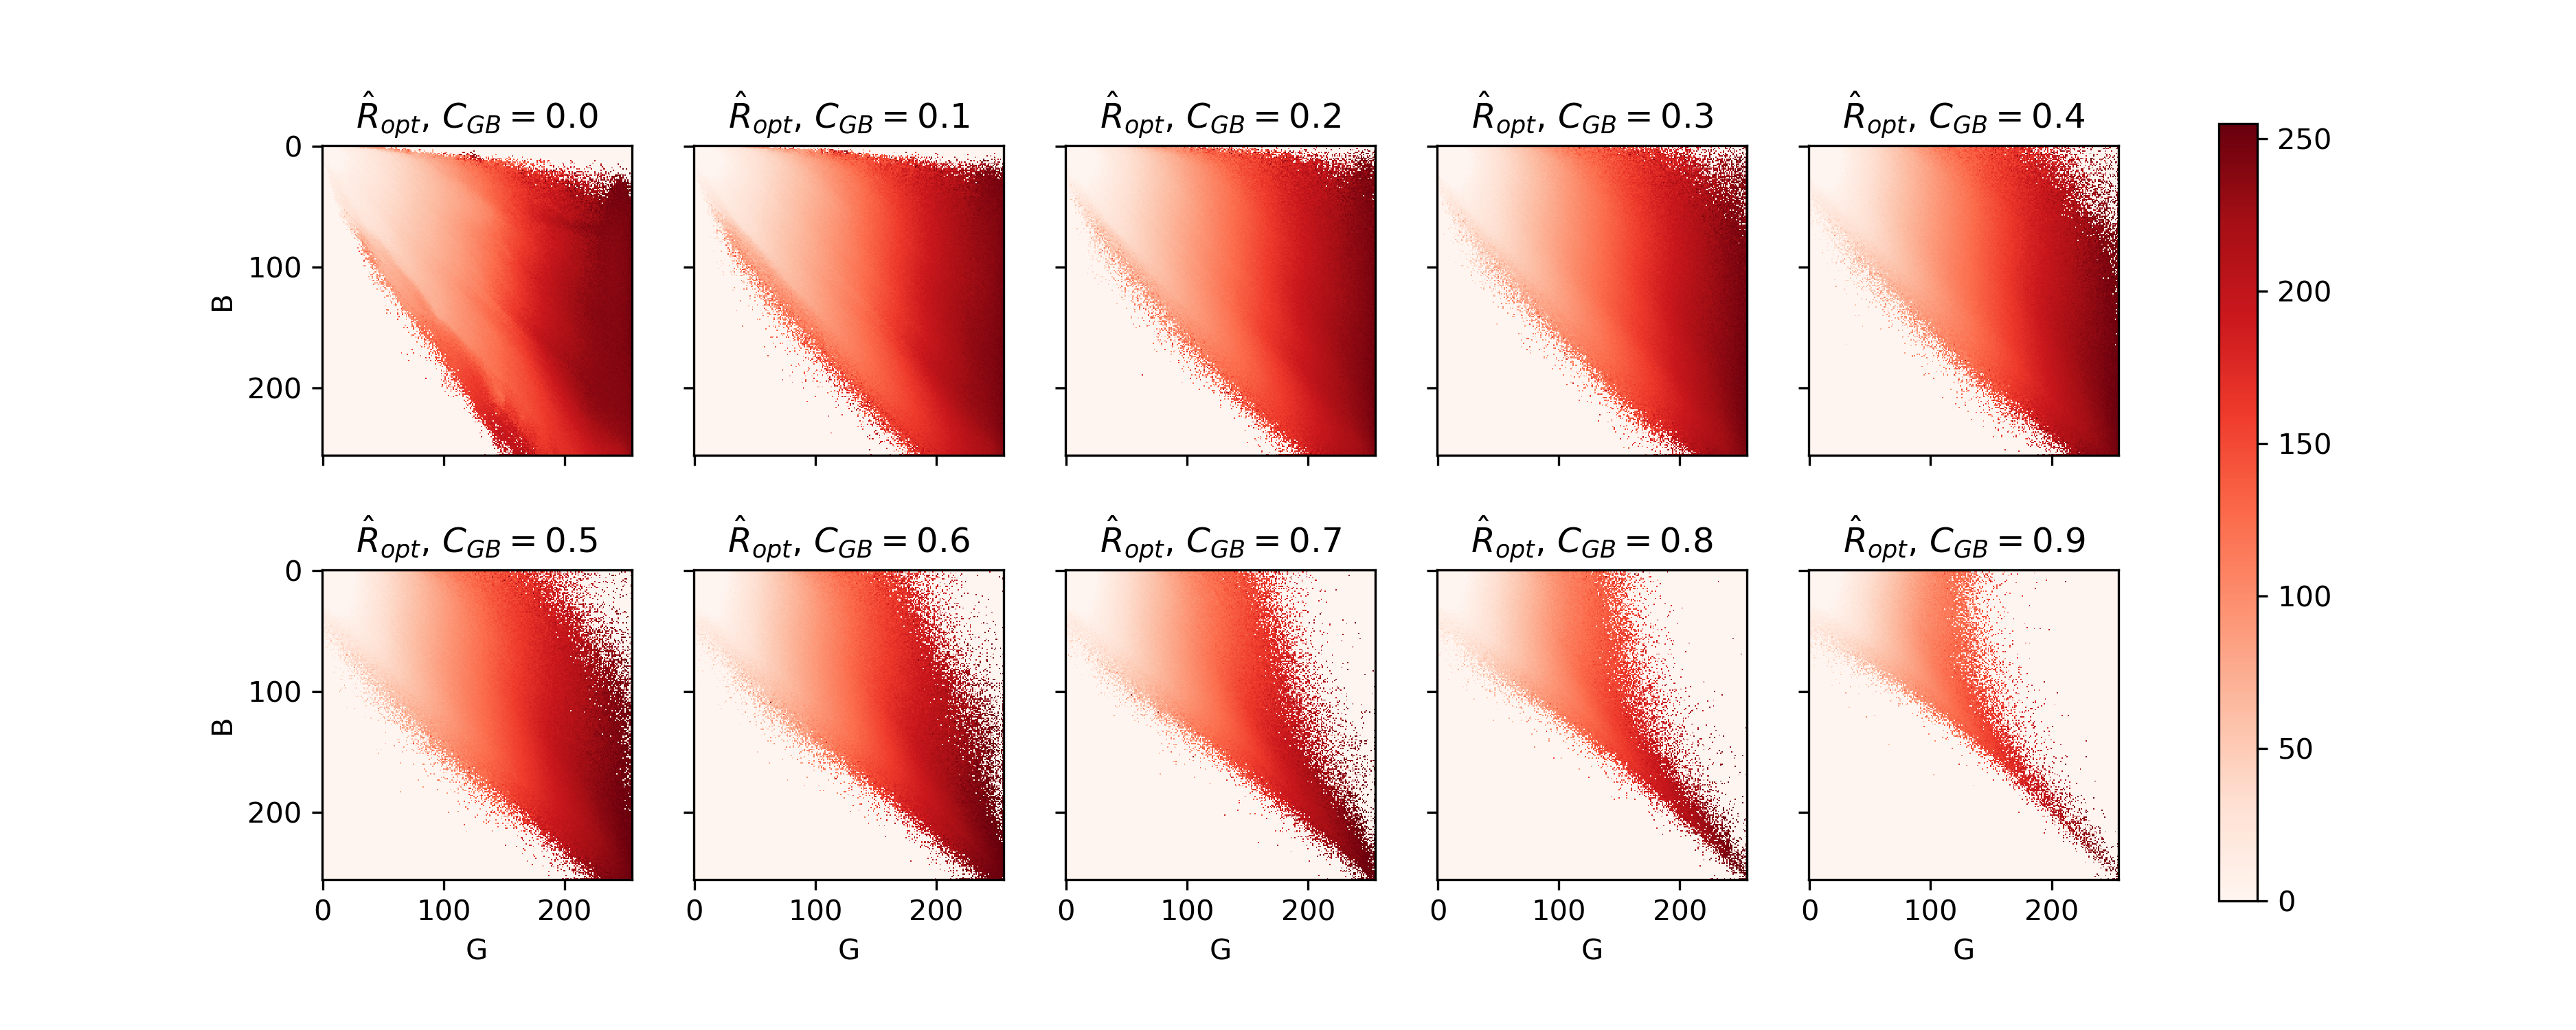
\includegraphics[width=1\columnwidth]{Figure/predicted_red} % Example image
	\caption{predicted red}
	\label{predicted red}
\end{figure}

\begin{figure}[h] % [h] forces the figure to be output where it is defined in the code (it suppresses floating)
	\centering
	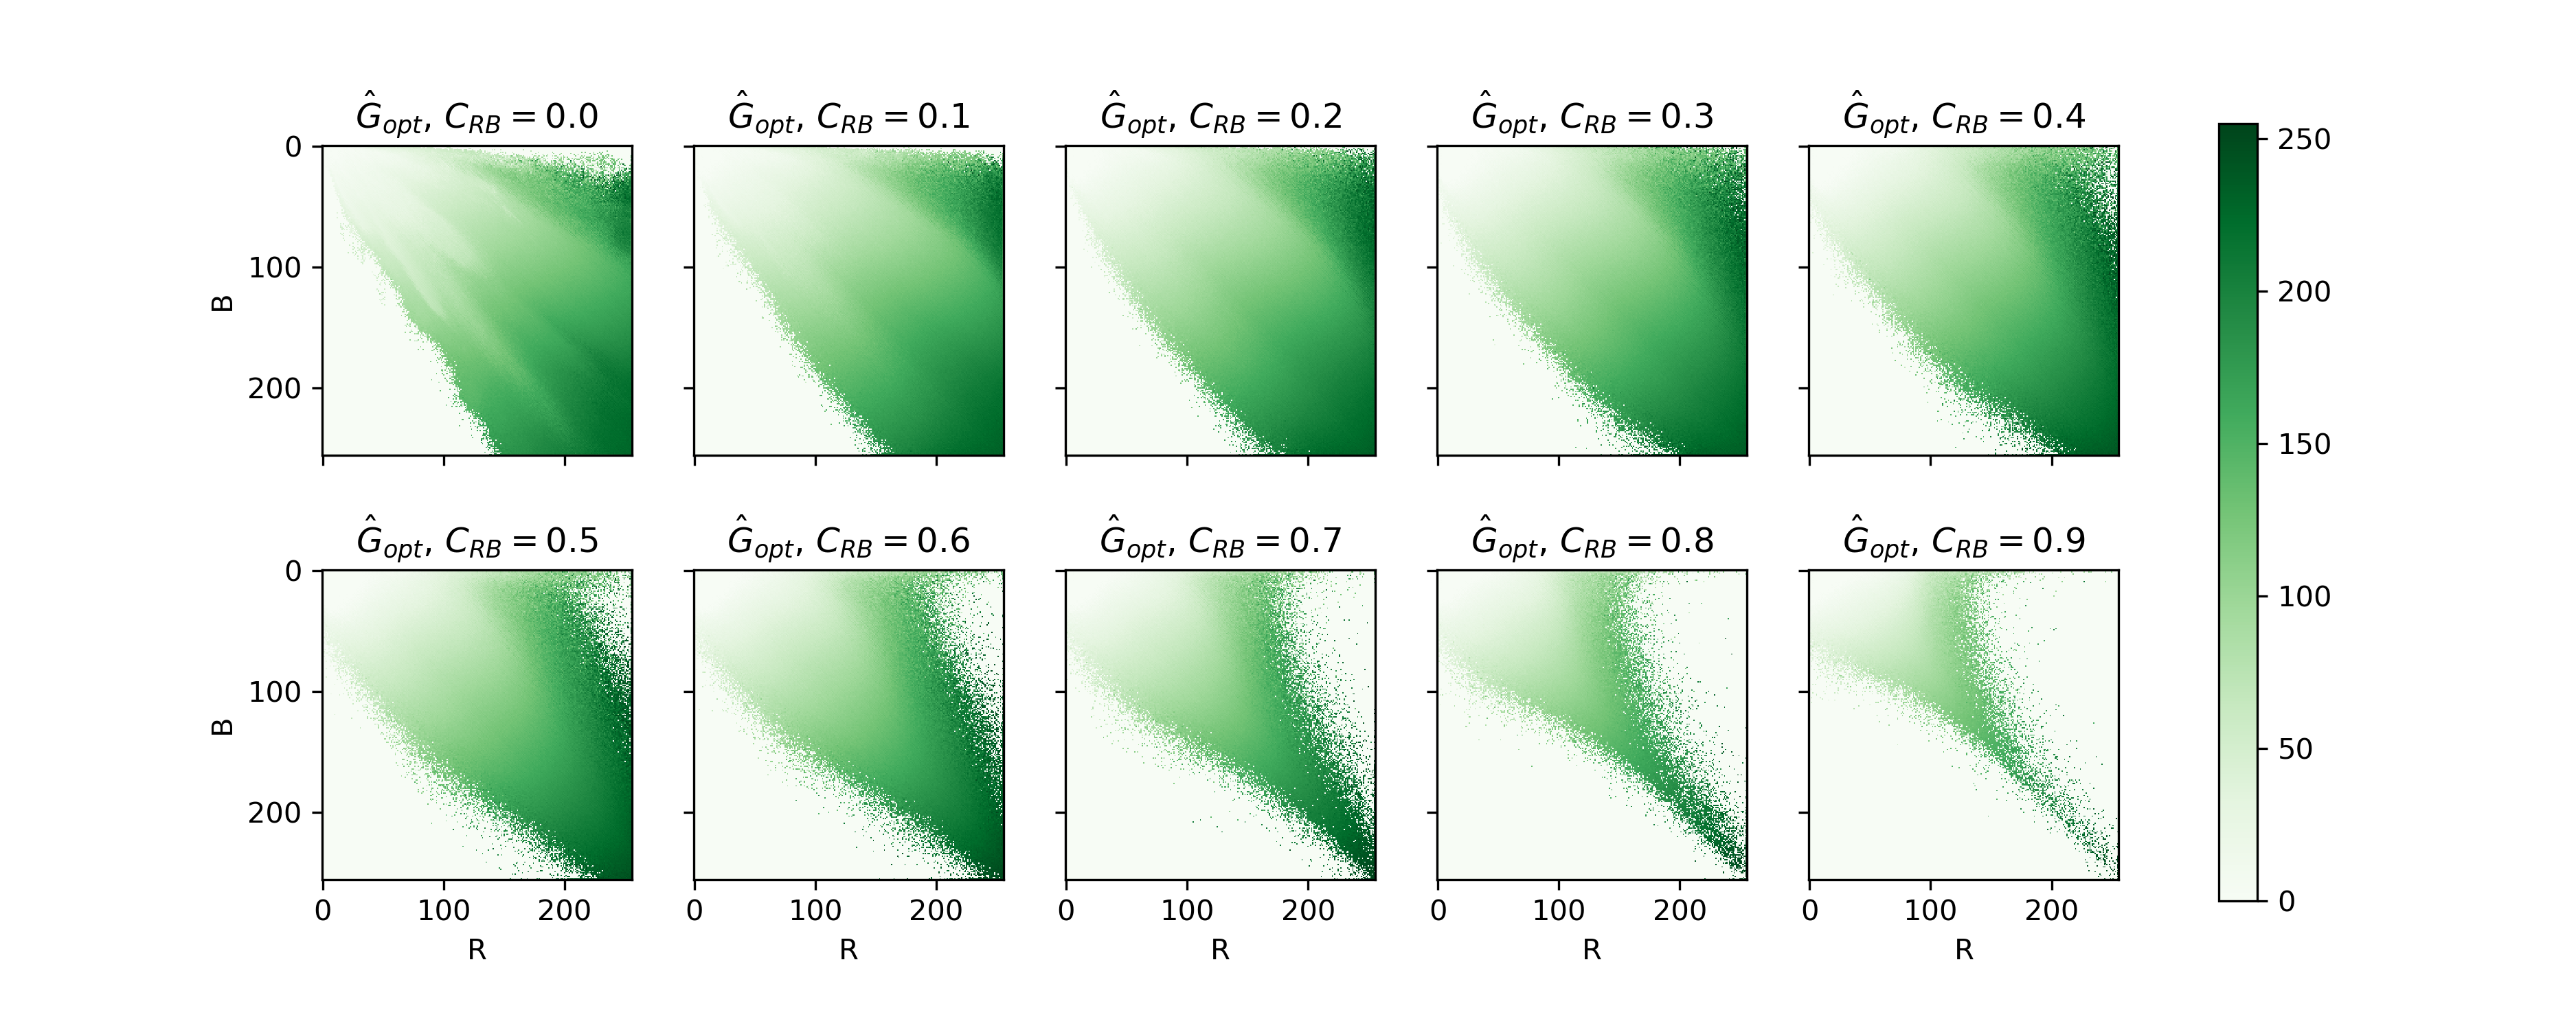
\includegraphics[width=1\columnwidth]{Figure/predicted_green} % Example image
	\caption{predicted green}
	\label{predicted green}
\end{figure}


\begin{figure}[h] % [h] forces the figure to be output where it is defined in the code (it suppresses floating)
	\centering
	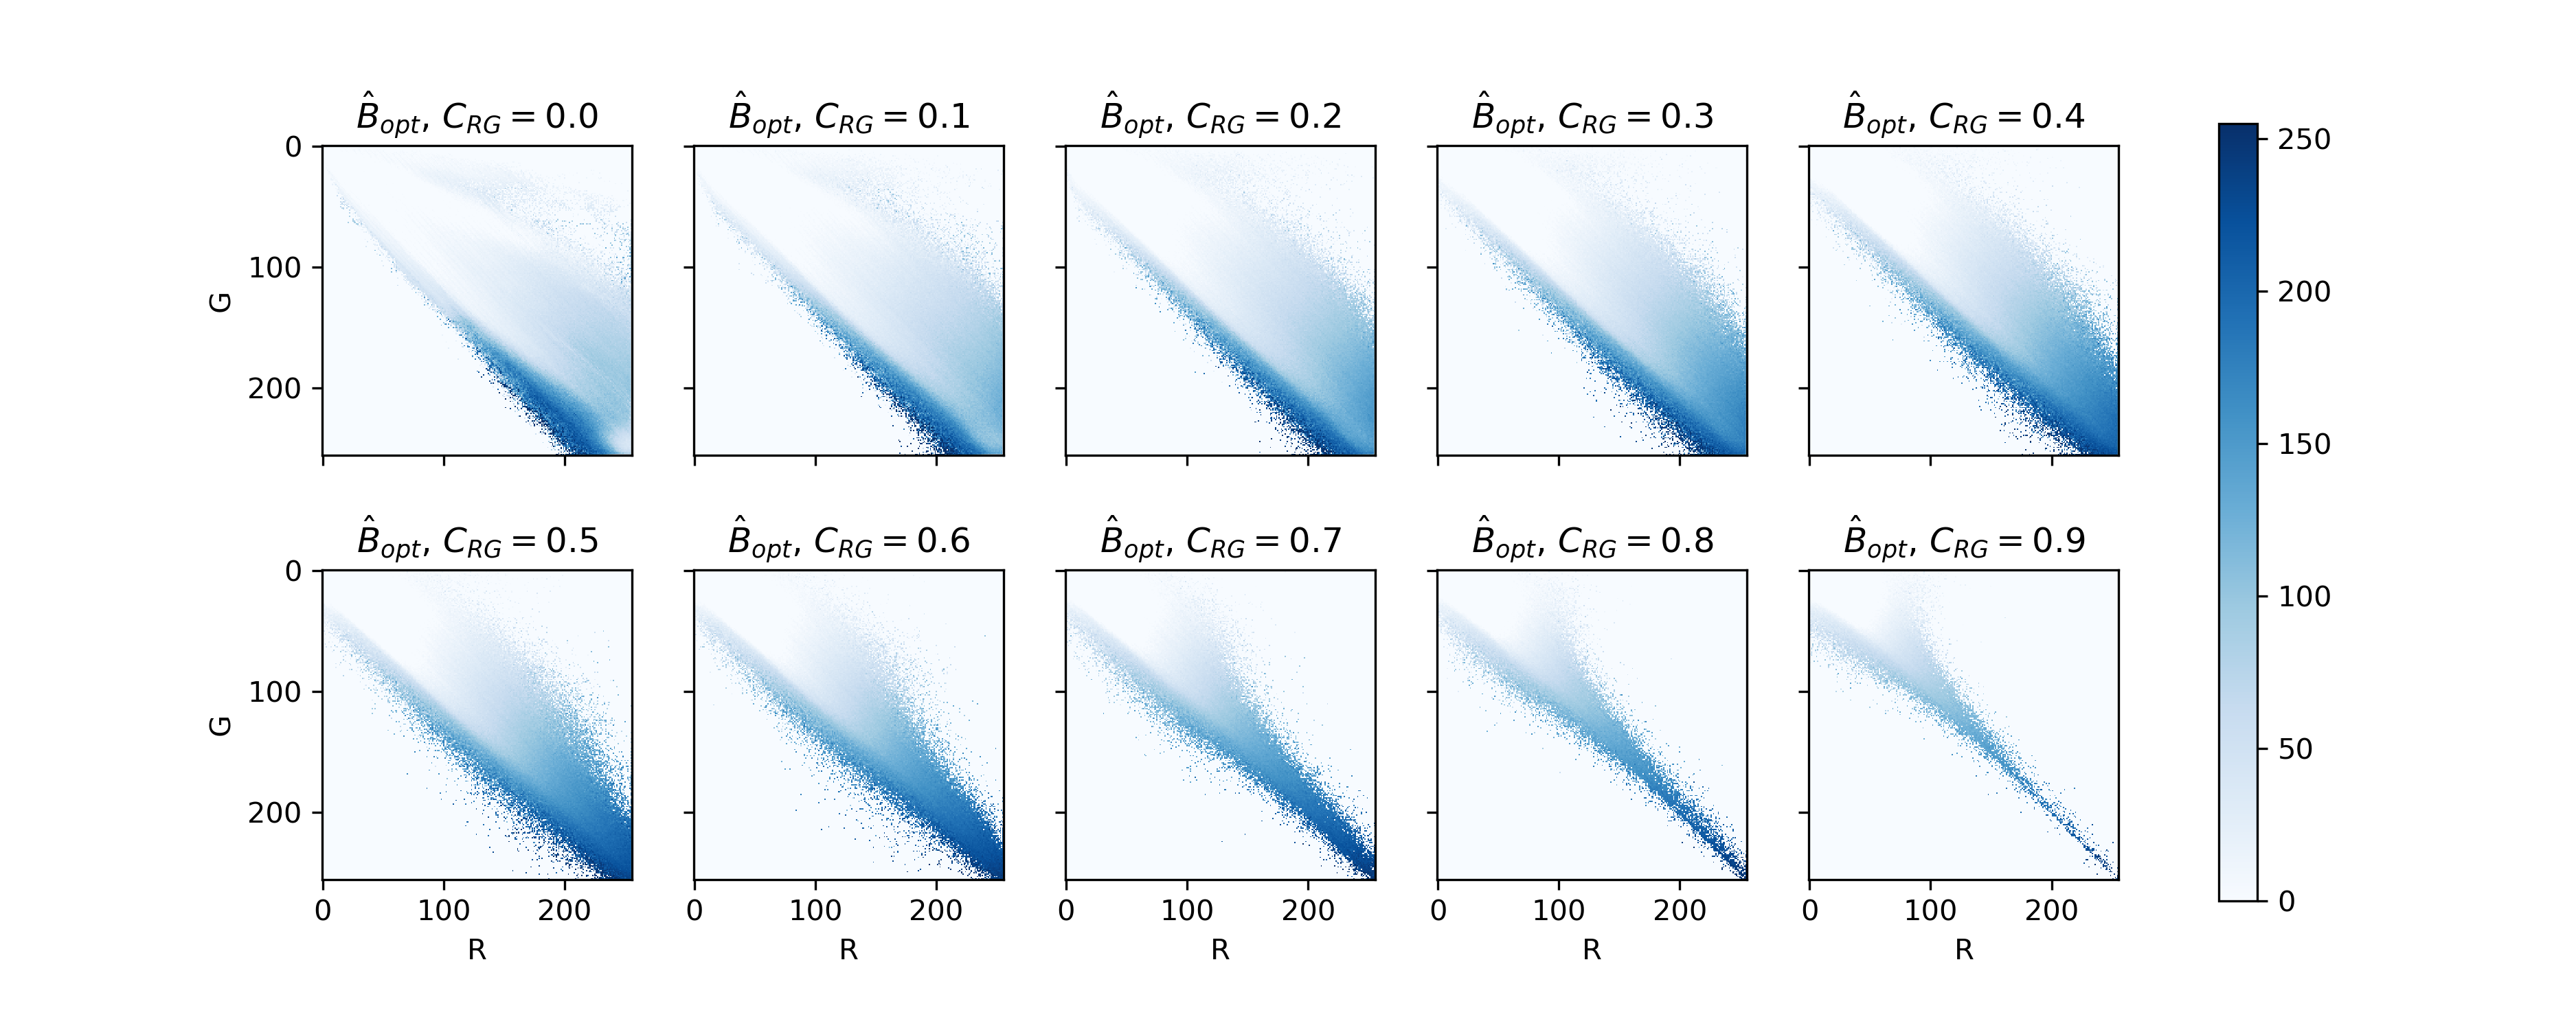
\includegraphics[width=1\columnwidth]{Figure/predicted_blue} % Example image
	\caption{predicted blue}
	\label{predicted blue}
\end{figure}

\begin{figure}[h] % [h] forces the figure to be output where it is defined in the code (it suppresses floating)
	\centering
	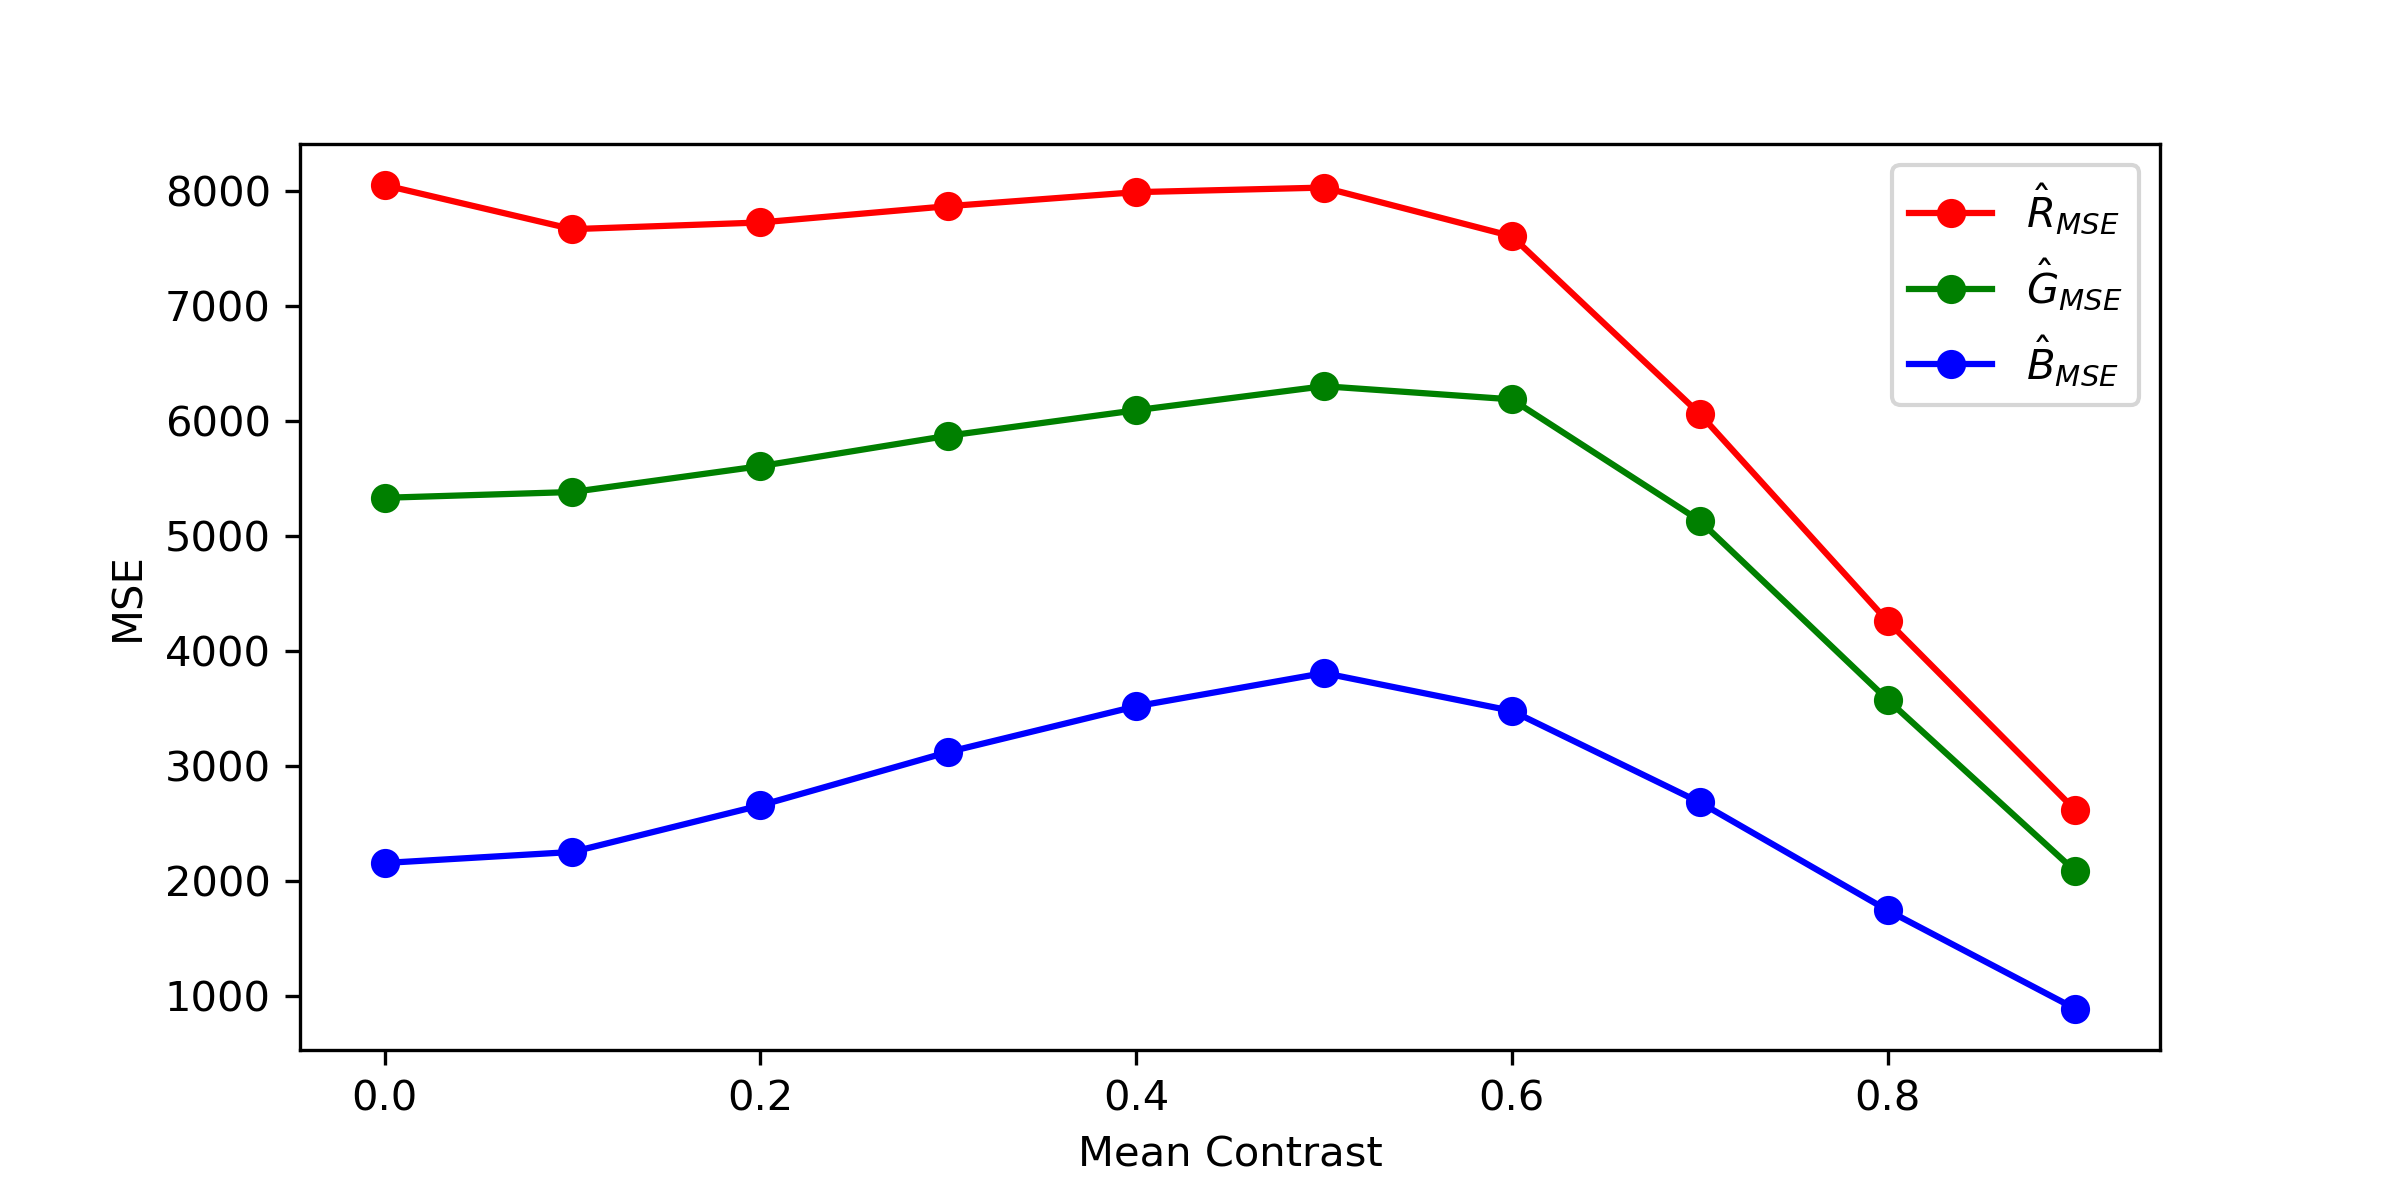
\includegraphics[width=1\columnwidth]{Figure/MSE_contrast} % Example image
	\caption{MSE contrast}
	\label{MSE}
\end{figure}

\begin{figure}[H]
	\centering  %图片全局居中
	\subfigure[predicted red no contrast]{
		\label{predicted_red_no_contrast}
		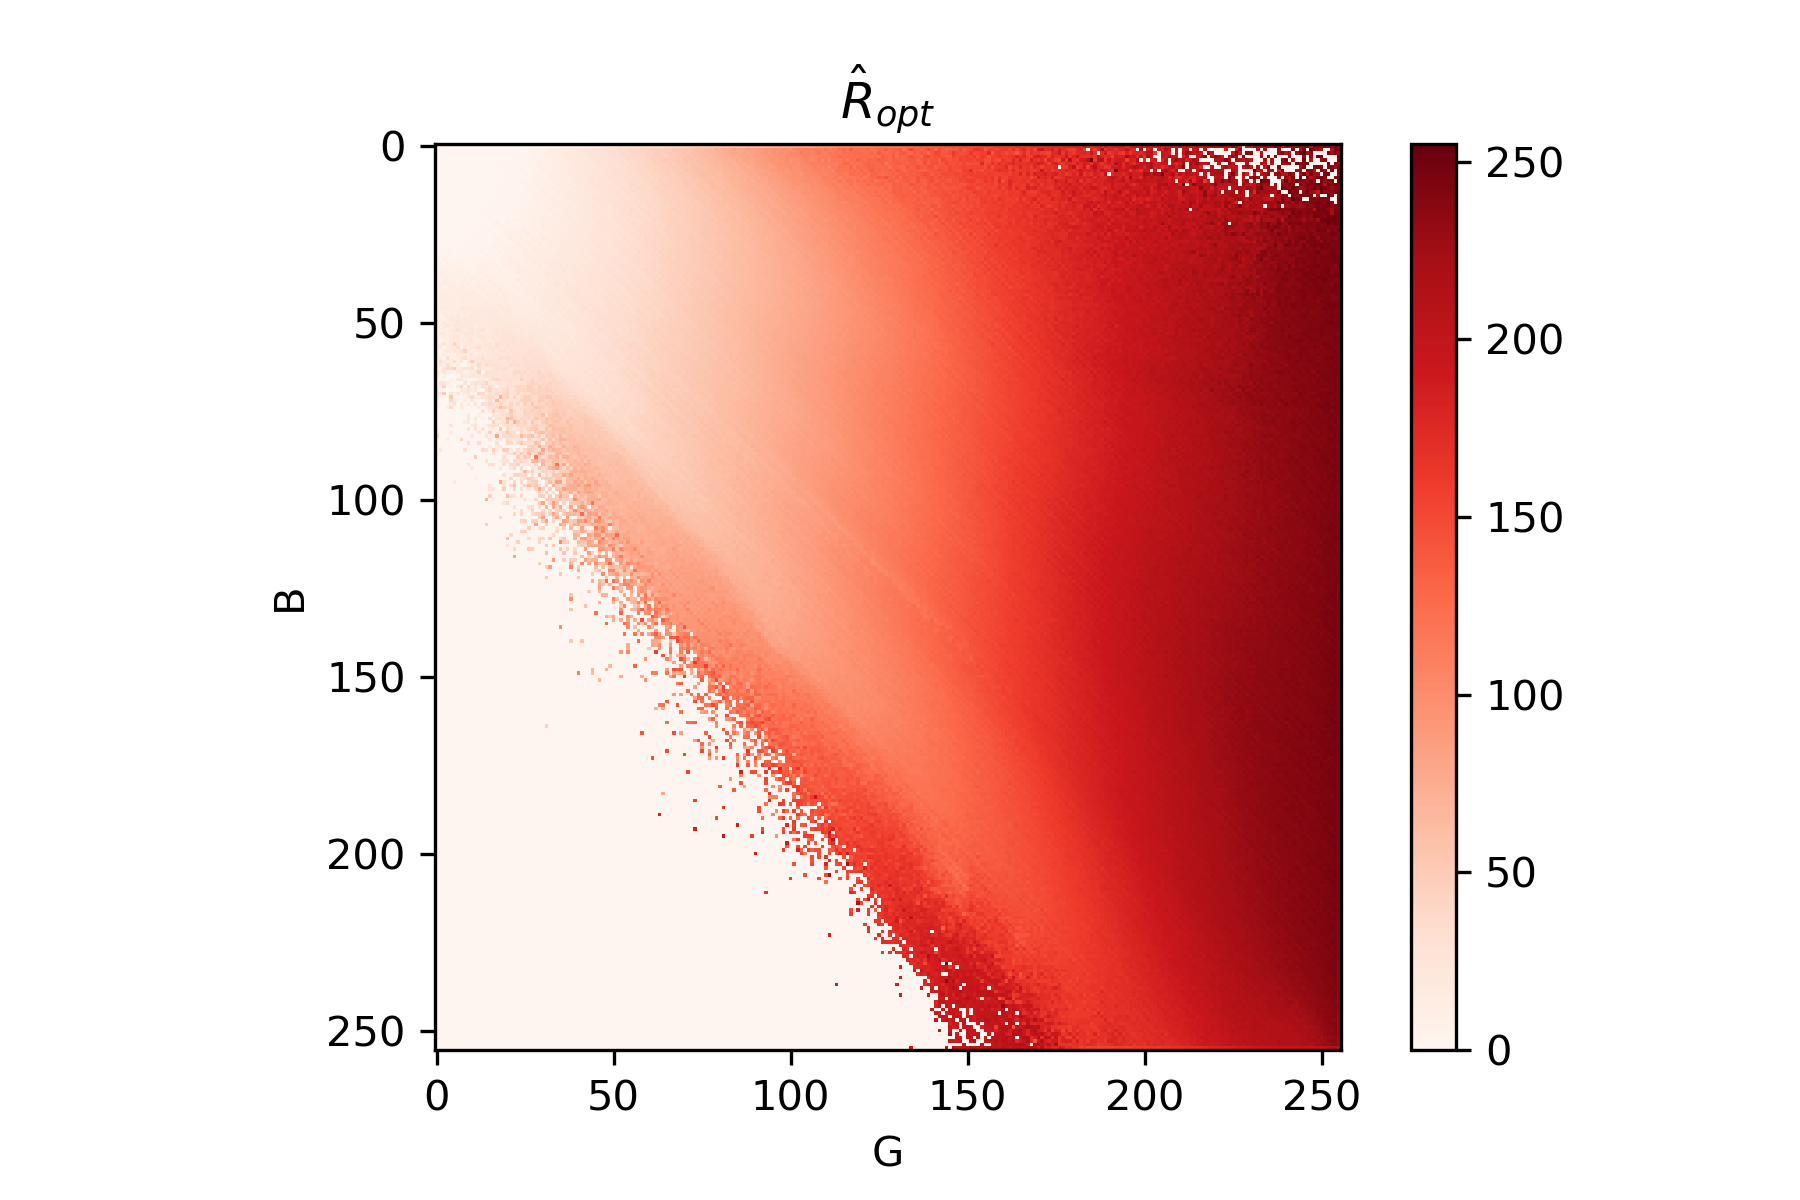
\includegraphics[width=0.32\textwidth]{Figure/predicted_red_no_contrast}}
	\subfigure[predicted green no contrast]{
		\label{predicted_green_no_contrast}
		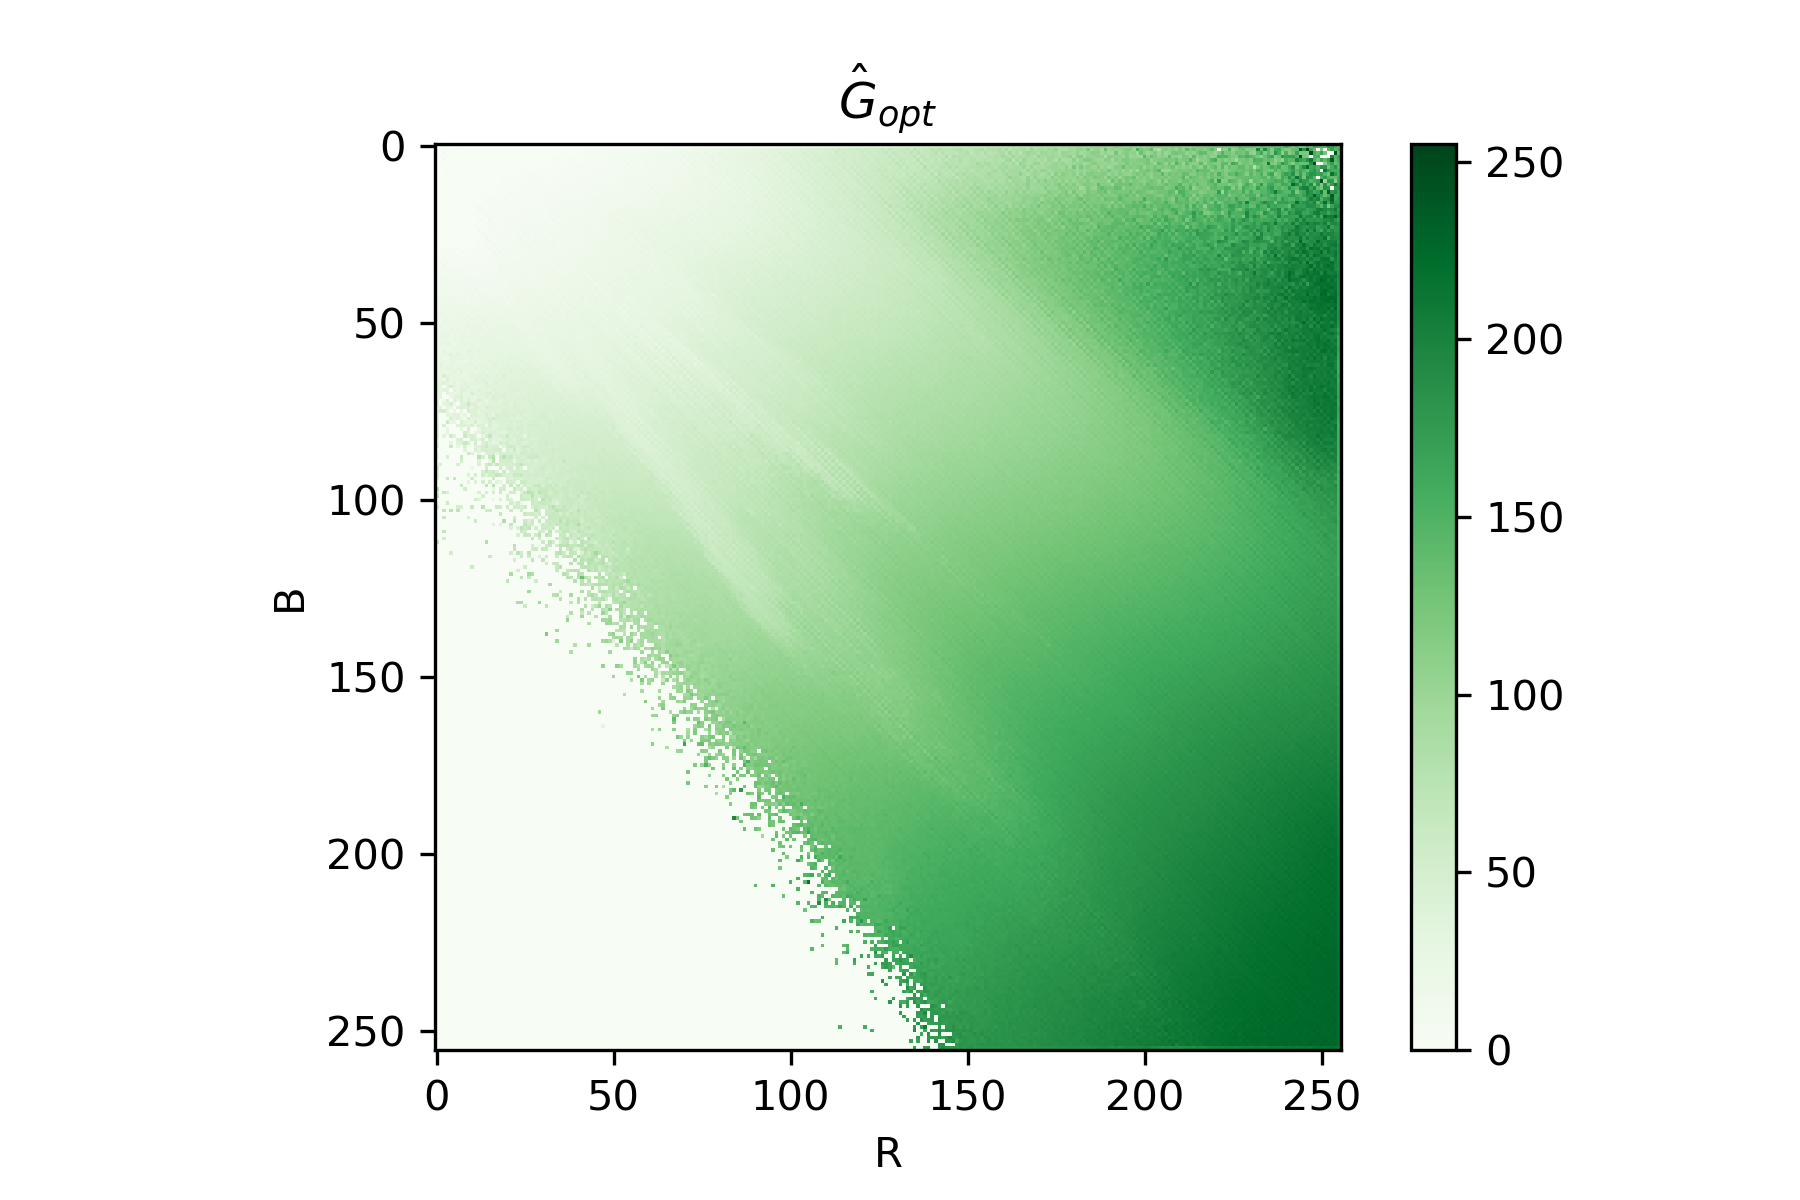
\includegraphics[width=0.32\textwidth]{Figure/predicted_green_no_contrast}}
	\subfigure[predicted blue no contrast]{
		\label{predicted_blue_no_contrast}
		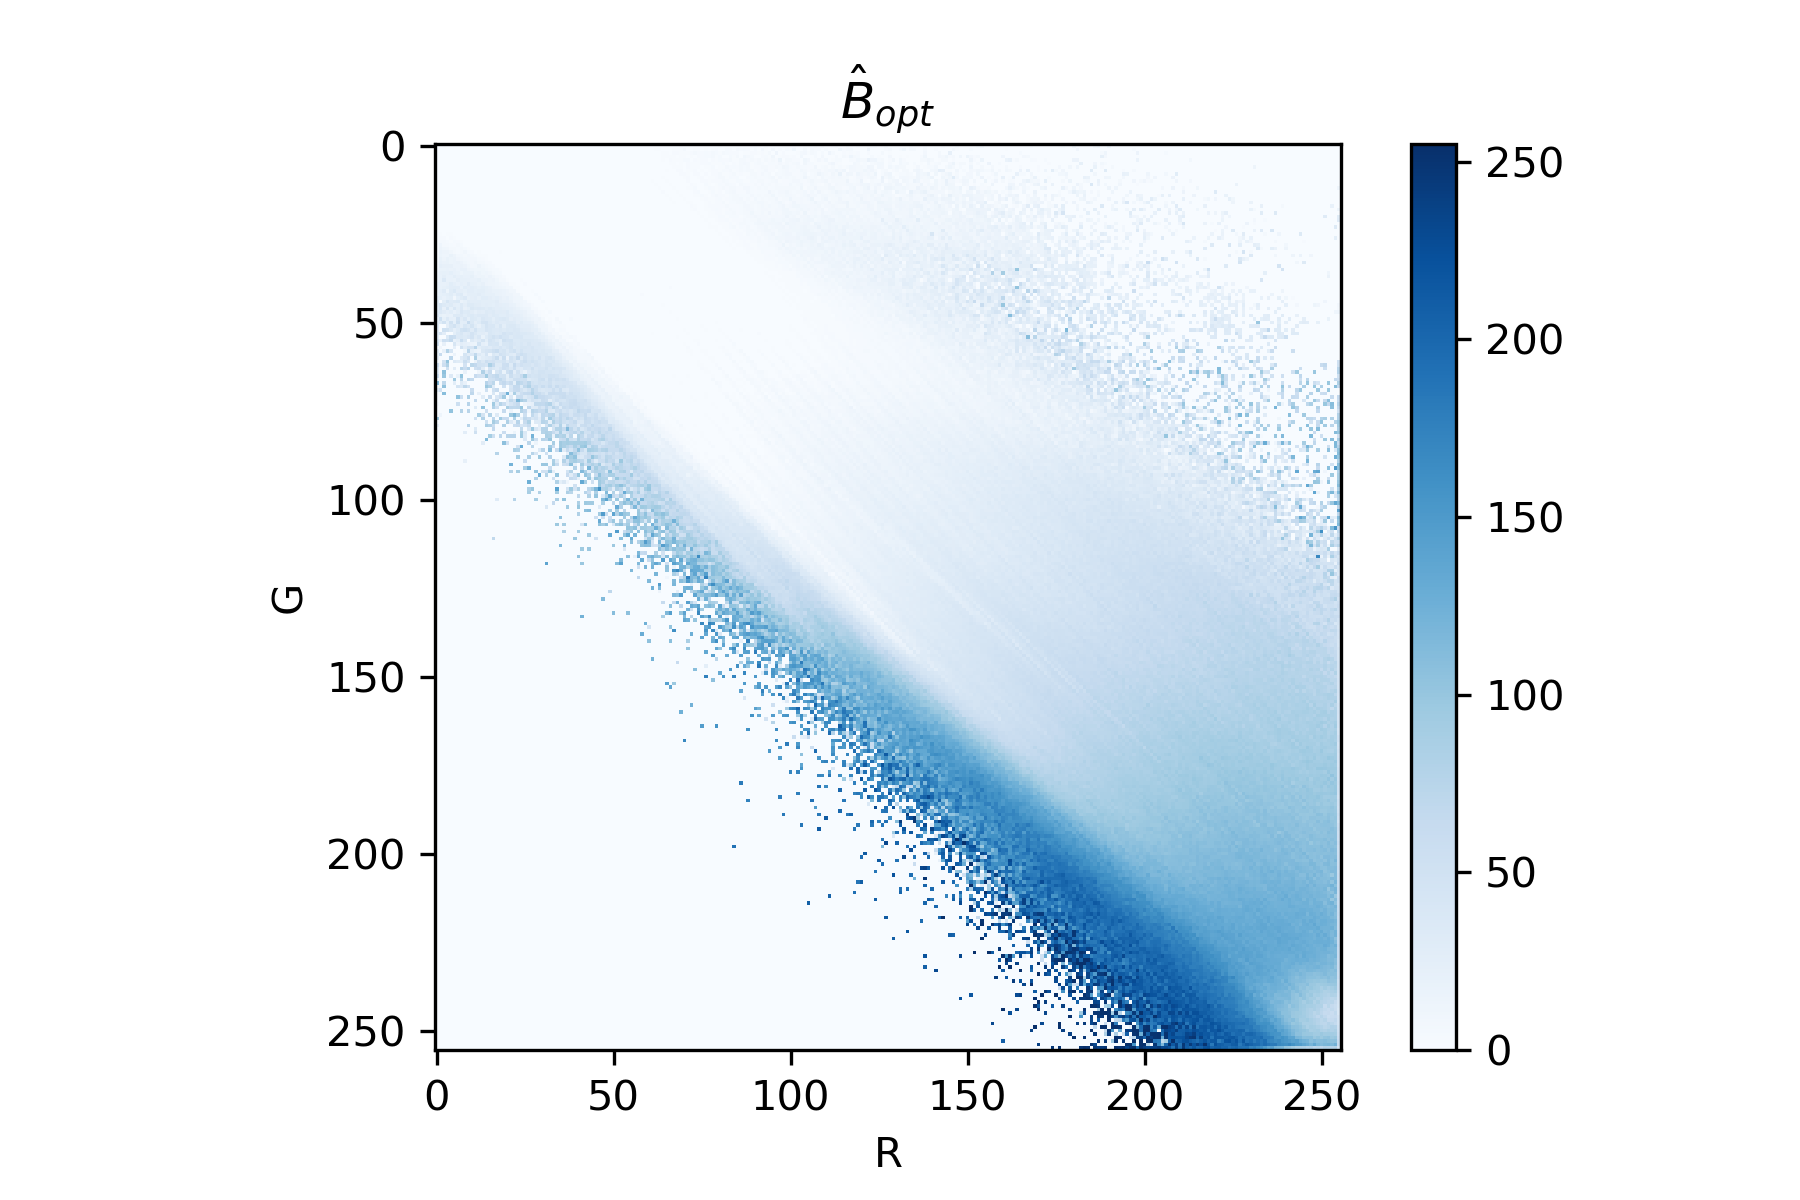
\includegraphics[width=0.32\textwidth]{Figure/predicted_blue_no_contrast}}
	\caption{predicted color no contrast}
	\label{predicted color no contrast}
\end{figure}

\begin{figure}[H]
	\centering  %图片全局居中
	\subfigure[predicted red no contrast surface plot]{
		\label{predicted_red_no_contrast_surf}
		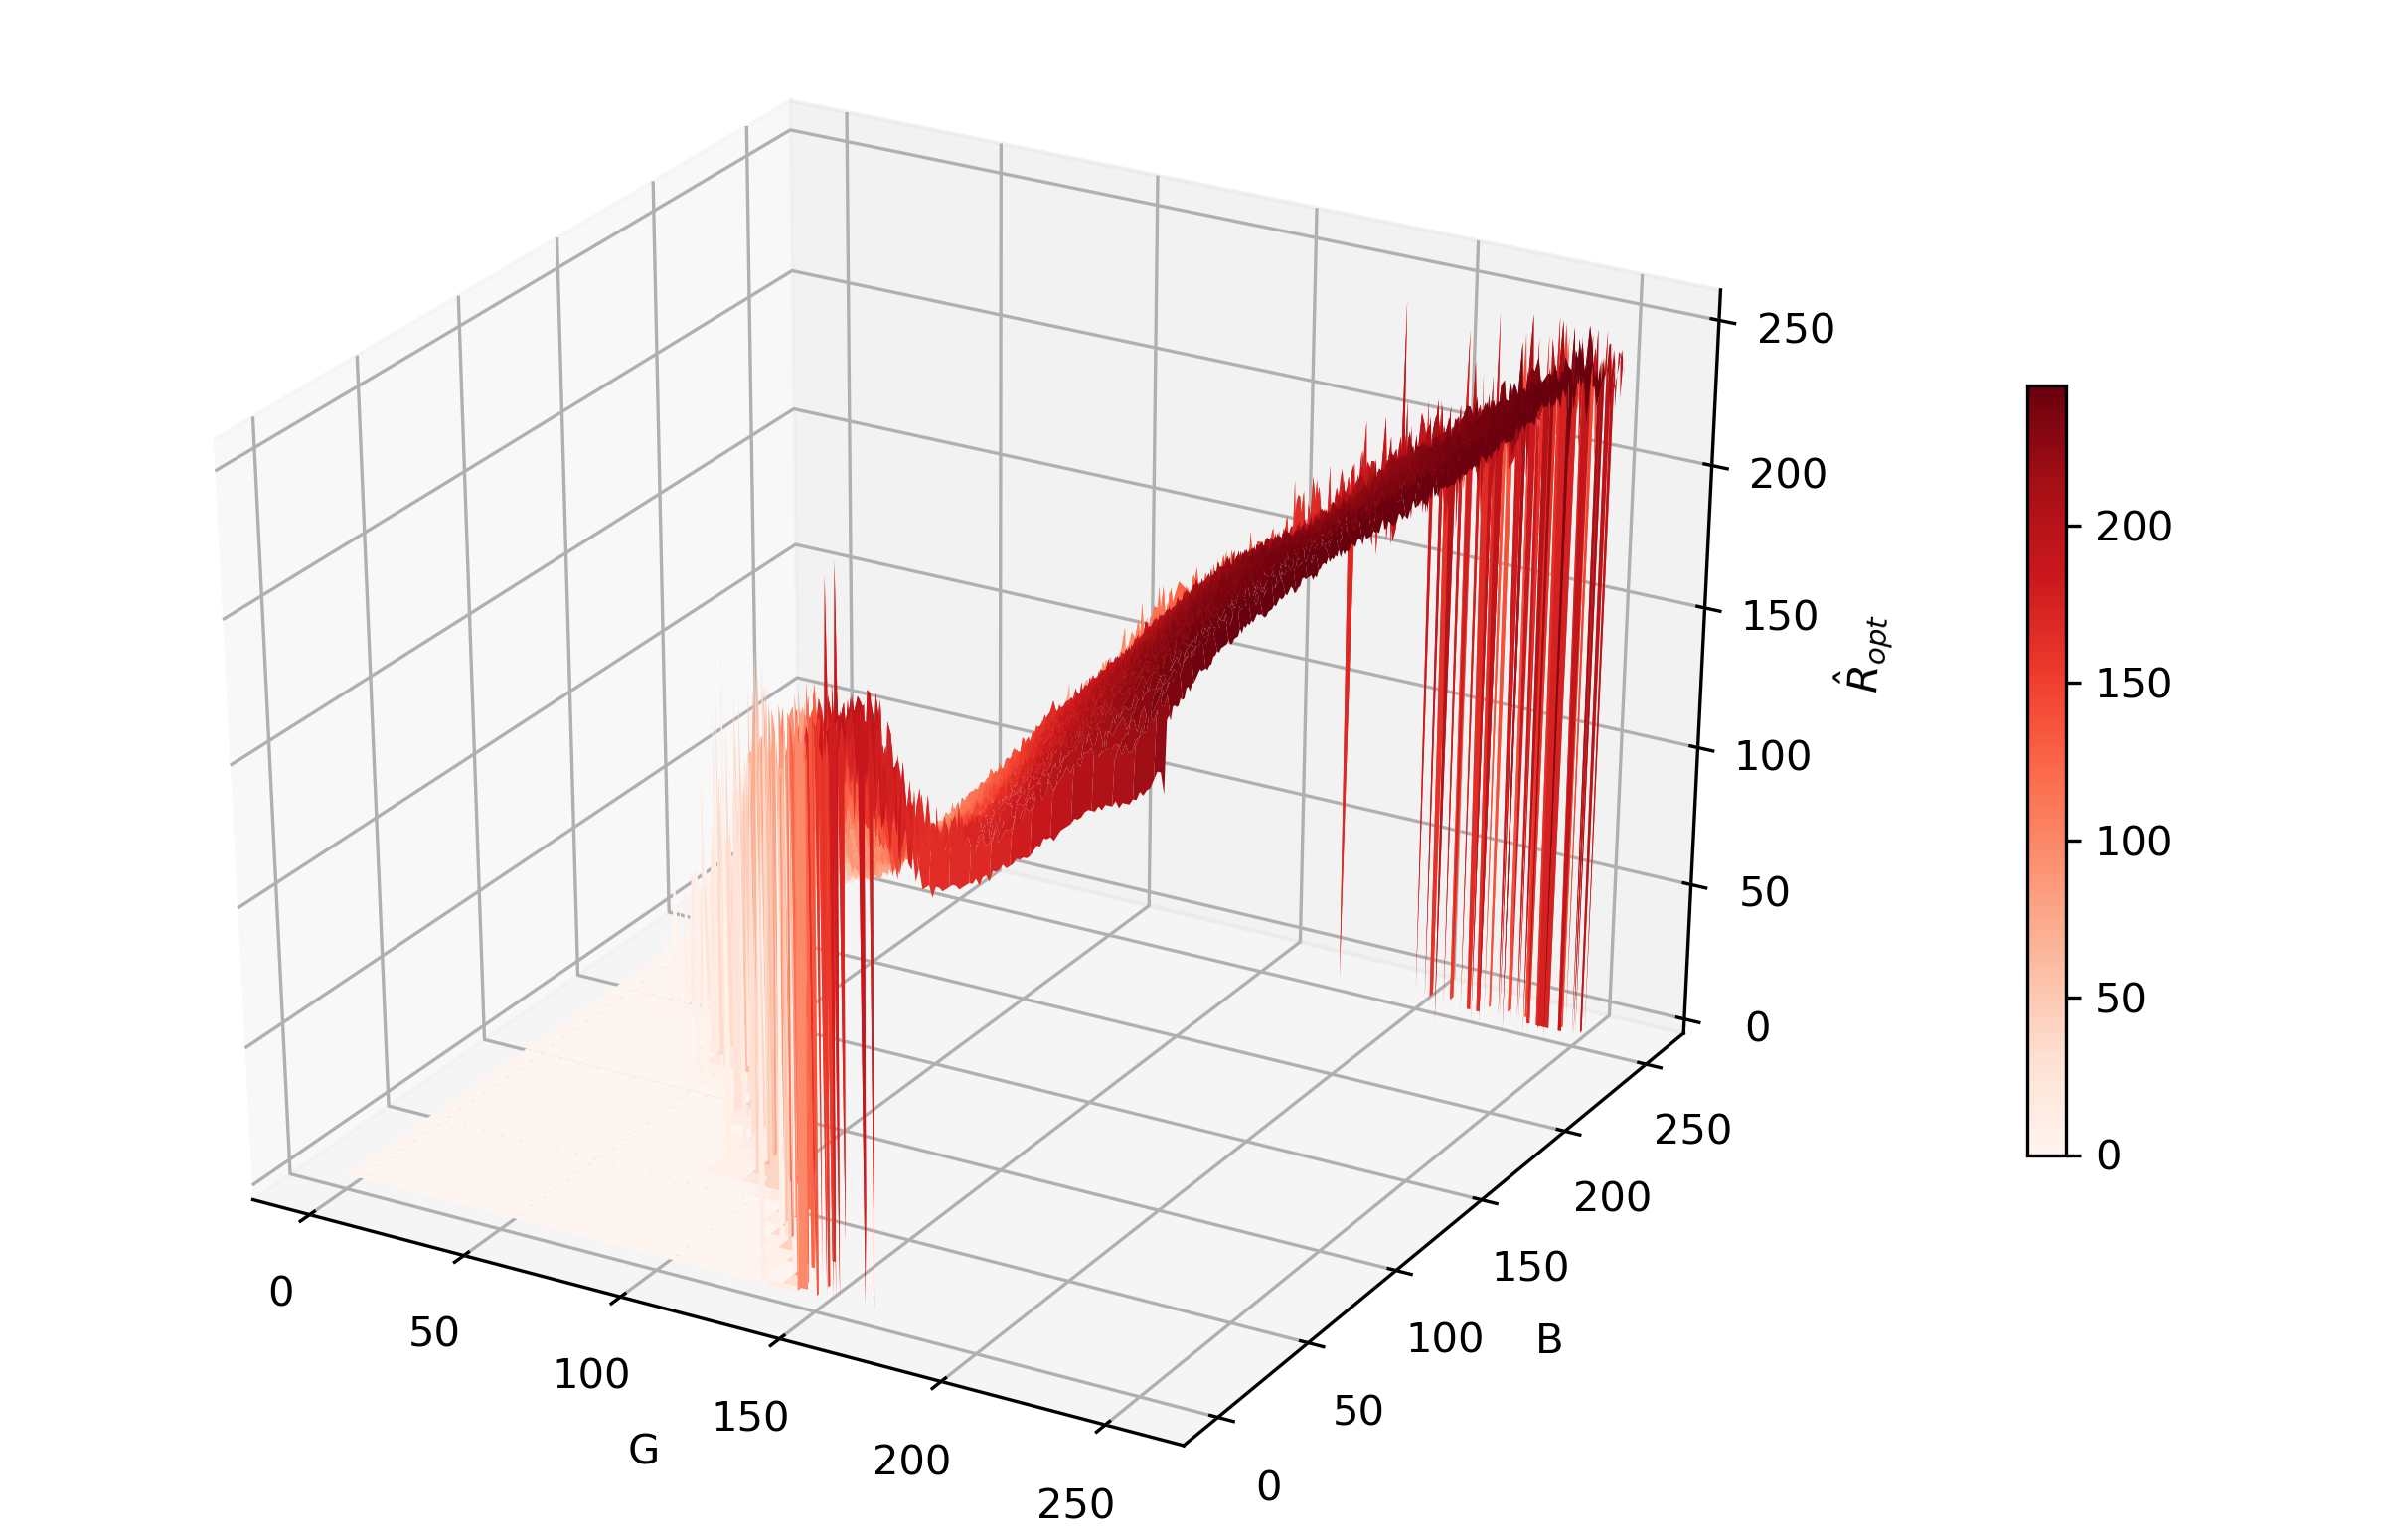
\includegraphics[width=0.32\textwidth]{Figure/predicted_red_no_contrast_surf}}
	\subfigure[predicted green no contrast surface plot]{
		\label{predicted_green_no_contrast_surf}
		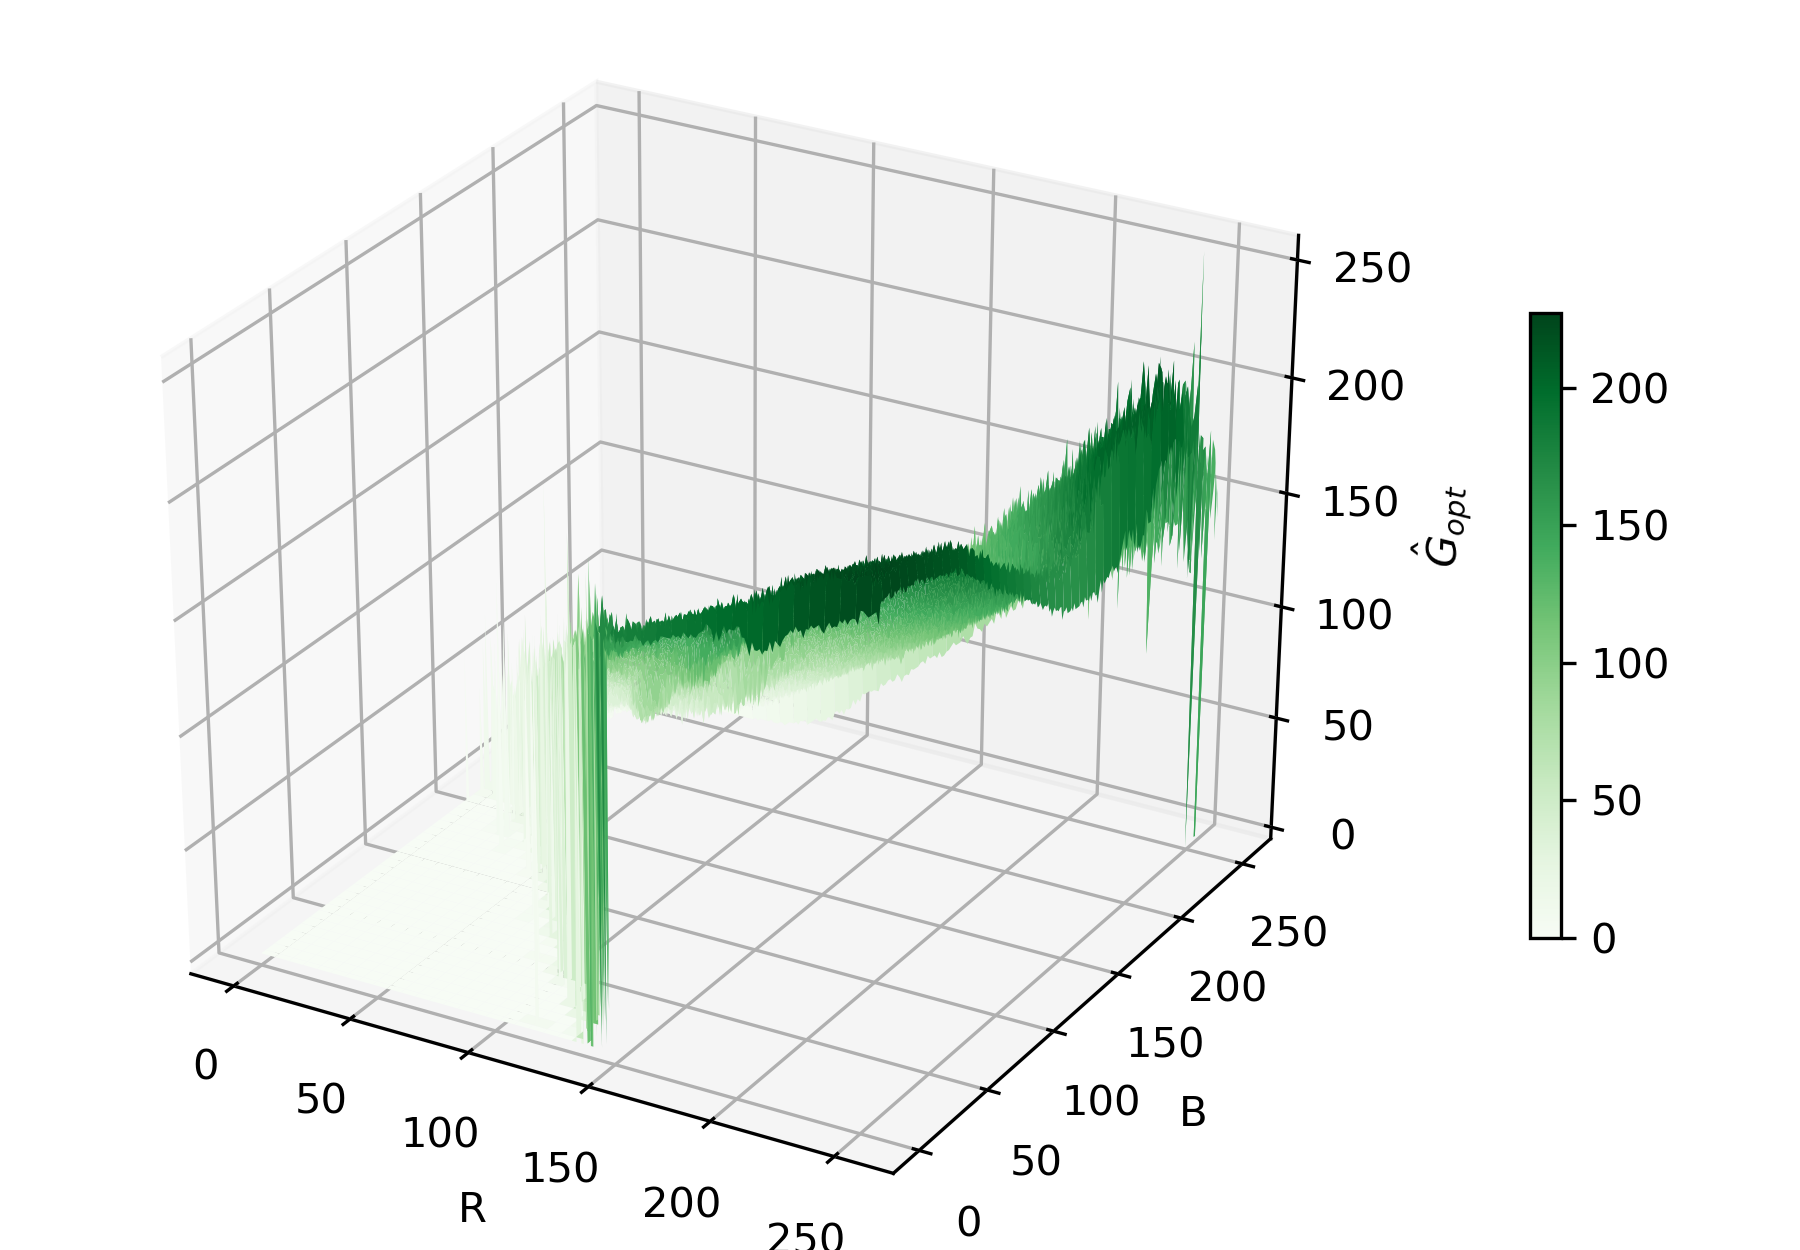
\includegraphics[width=0.32\textwidth]{Figure/predicted_green_no_contrast_surf}}
	\subfigure[predicted blue no contrast surface plot]{
		\label{predicted_blue_no_contrast_surf}
		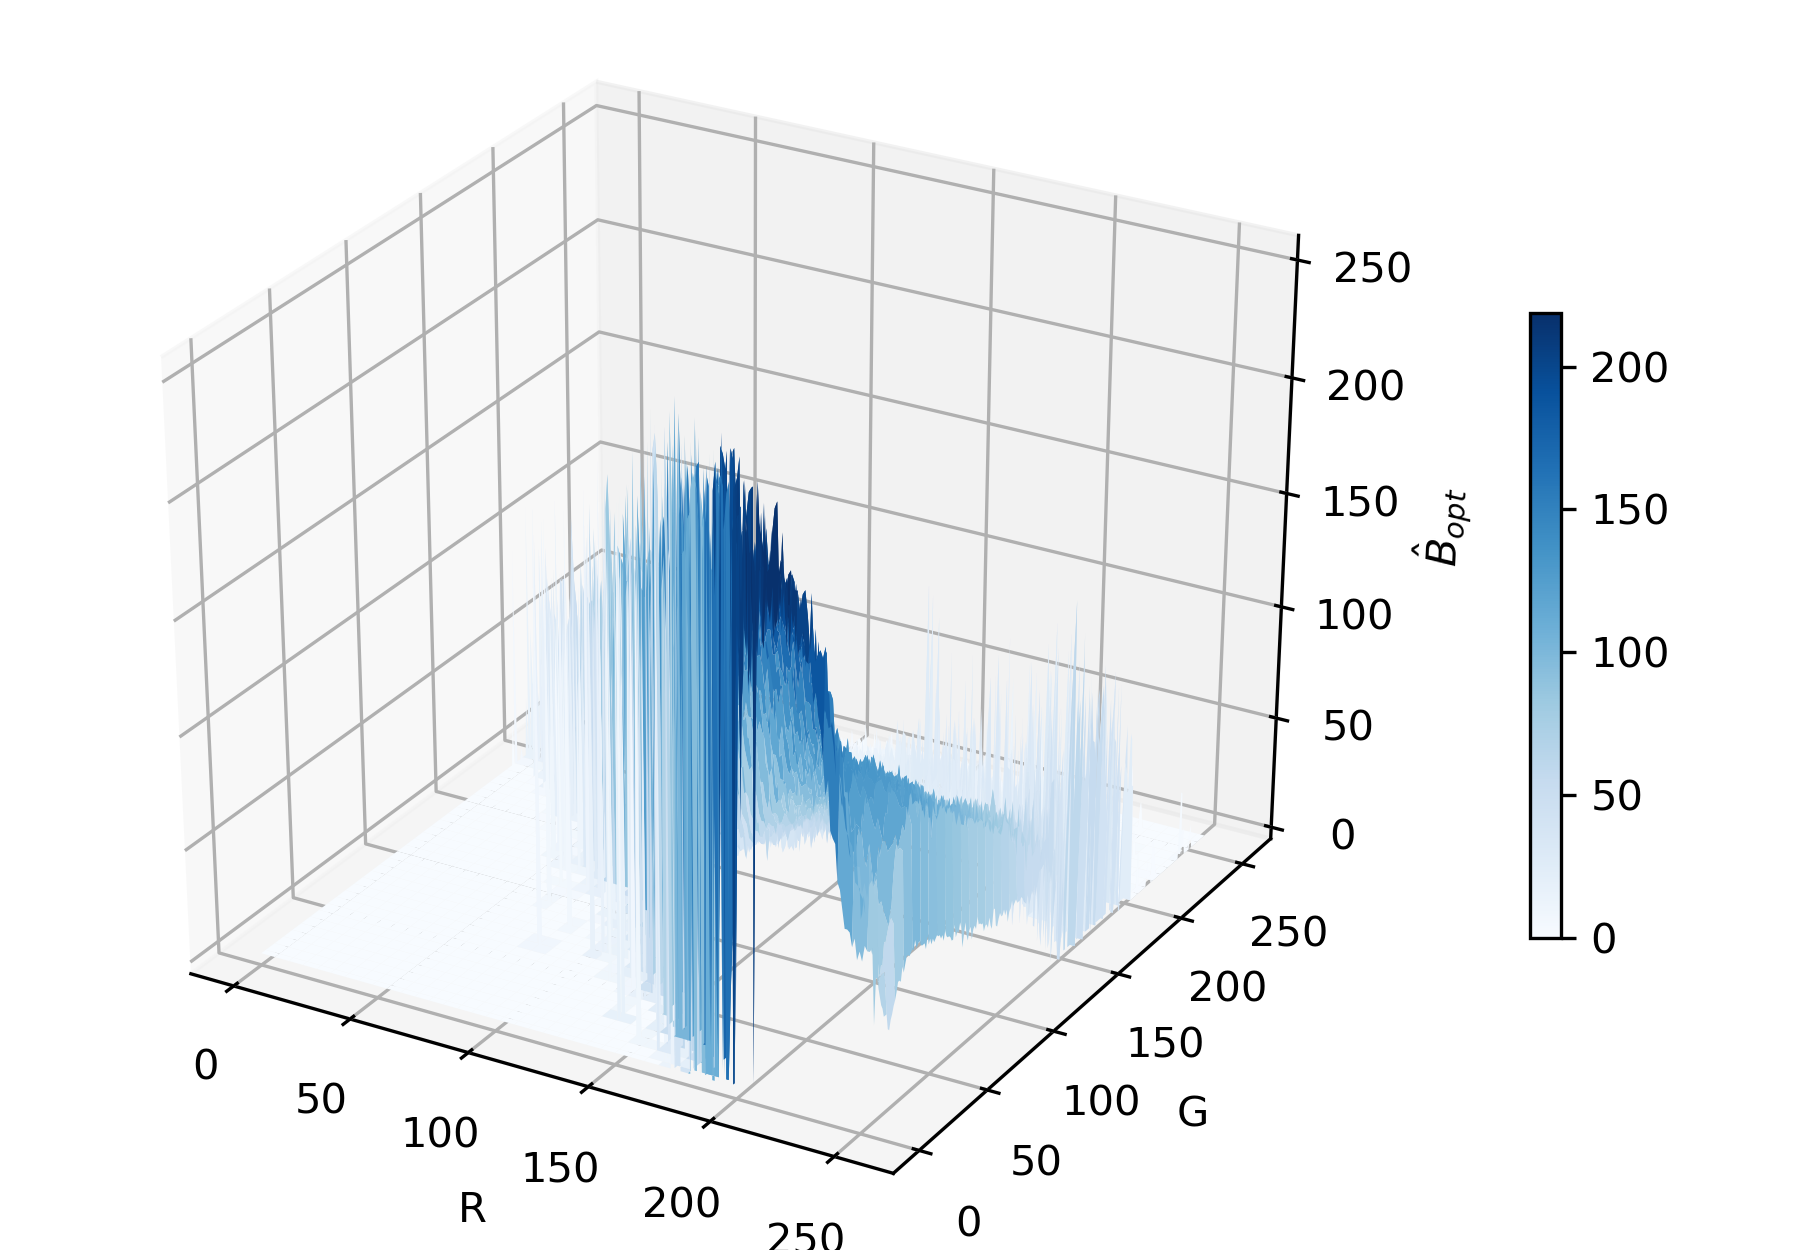
\includegraphics[width=0.32\textwidth]{Figure/predicted_blue_no_contrast_surf}}
	\caption{predicted color no contrast}
	\label{predicted color no contrast surface plot}
\end{figure}

\subsection{Recover images}

%cps201004281214 recover \ref{cps201004281214_recover}
%cps201004291795 recover \ref{cps201004291795_recover}
%\begin{figure}[h] % [h] forces the figure to be output where it is defined in the code (it suppresses floating)
%	\centering
%	\includegraphics[width=1\columnwidth]{Figure/cps201004281214_recover} % Example image
%	\caption{cps201004281214 recover}
%	\label{cps201004281214_recover}
%\end{figure}

%\begin{figure}[h] % [h] forces the figure to be output where it is defined in the code (it suppresses floating)
%	\centering
%	\includegraphics[width=1\columnwidth]{Figure/cps201004291795_recover} % Example image
%	\caption{cps201004291795 recover}
%	\label{cps201004291795_recover}
%\end{figure}

\subsubsection{Experiment 3}

In this experiment we set learning rate as 0.01 and the number of units in hidden layer is 100 and smaller initiation of $W$ and $b$ ($W_{ij}, b_i \sim N(0,0.01)$). The result is shown as \ref{SGD_training_lr001_wb001} and \ref{SGD_testing_SGD001_wb001}. We can find that the loss converges after several thousands iterations but it fluctuate drastically after that. The accuracy is 92.09\%.



\subsubsection{Accuracy}

We set iteration of 60000 times and learning rate as 0.1. We try different number of units in hidden layer to see its influence on accuracy.

The accuracy is shown as \ref{SGD_accuracy}, from which we can find arond 100 neurons performs reletivaly well.


\subsubsection{Accuracy of ReLU}
Here we built a neural network with one hidden layer and applied SGD and ReLU as activation function. We iterate 60000 times, i.e. go over all training images once. earning rate as 0.1 and $W_{ij}, b_i \sim N(0,0.1)$. The result of accuracy is shown as \ref{SGD_relu_accuracy}. We can find the accuracy is less than that of sigmoid and unstable.



%----------------------------------------------------------------------------------------
%	LIST EXAMPLES
%----------------------------------------------------------------------------------------

\section{Conclusion}

In this report, we built a neural network with only 1 hidden layer and we can see the accuracy can approach more than 95\%. However, there are some problems need to be solved, like the loss obtained from SGD is not stable. What's more, comparing sigmoid and ReLU, we find that sigmoid behaves better than ReLU and the reason is unclear.

\paragraph{next step}
SGD is not stable, I may use gradient descent and batch gradient descent to see if they are more stable. I can try other activation functions and add more hidden layers. In addition, I write this neural network by myself. I should learn some packages like tensorflow, pytorch to build networks.


%----------------------------------------------------------------------------------------

\end{document}
